\documentclass[11pt]{article}

\usepackage[margin=1.1in]{geometry}
\usepackage{amsmath,amssymb,amsthm}
\usepackage{booktabs}
\usepackage{graphicx}
\usepackage{fancyhdr}
\usepackage[colorlinks=true,linkcolor=blue,citecolor=blue,urlcolor=blue]{hyperref}
\hypersetup{
  pdftitle={Properly colored paths in the union of two Hamiltonian paths: the O(sqrt n) collapse, the transit floor, and the failure of block lower bounds},
  pdfauthor={Alejandro Lizardi},
  pdfsubject={Combinatorics; properly colored paths in edge-colored multigraphs},
  pdfkeywords={properly colored path; alternating path; edge-colored multigraph; union of Hamiltonian paths; permutation; inflation; transit number; scrambled ladder}
}

% ----- Periapsis branding (house style) -------------------------------------
% Plain page numbers in the footer; no footer mark.
\pagestyle{fancy}
\fancyhf{}
\renewcommand{\headrulewidth}{0pt}
\renewcommand{\footrulewidth}{0pt}
\fancyfoot[C]{\footnotesize\thepage}
\fancypagestyle{plain}{% so page 1 (\maketitle uses 'plain') carries the footer too
  \fancyhf{}\renewcommand{\headrulewidth}{0pt}\renewcommand{\footrulewidth}{0pt}%
  \fancyfoot[C]{\footnotesize\thepage}}

\newtheorem{theorem}{Theorem}[section]
\newtheorem{lemma}[theorem]{Lemma}
\newtheorem{proposition}[theorem]{Proposition}
\newtheorem{corollary}[theorem]{Corollary}
\newtheorem{conjecture}[theorem]{Conjecture}
\theoremstyle{definition}
\newtheorem{definition}[theorem]{Definition}
\newtheorem{remark}[theorem]{Remark}
\newtheorem{observation}[theorem]{Observation}
\newtheorem{example}[theorem]{Example}

\newcommand{\pmin}{\rho_{\min}}
\newcommand{\pminK}[1]{\rho_{\min}^{(#1)}}
\newcommand{\inv}[1]{#1^{-1}}
\newcommand{\smax}{s_{\max}}
\DeclareMathOperator{\pc}{pc}

\title{Properly colored paths in the union of two Hamiltonian paths:\\
the $O(\sqrt{n}\,)$ collapse, the transit floor,\\
and the failure of block lower bounds}
\author{Alejandro Lizardi%
\thanks{Independent researcher, \texttt{alejlizardi05@gmail.com}.
The proofs and computations in this paper were AI-assisted by Claude, under the
Periapsis research structure. All computational claims are reproducible from the
ancillary files accompanying this submission; see Appendix~\ref{sec:comp}.}}
\date{July 2026}

\begin{document}
\maketitle

\begin{center}
  
\includegraphics[height=20pt]{assets/lockup.png}
\end{center}
\vspace{4pt}

\begin{abstract}
Overlay two Hamiltonian paths on a common vertex set of size $n$, one blue and one
red. How long a properly colored path -- consecutive edges alternating in color --
must the union contain? Every such union is $H_\sigma$ for a permutation $\sigma$ of
$\{0,\dots,n-1\}$, with blue edges joining consecutive positions and red edges
consecutive values; write $\rho(\sigma)$ for the maximum number of vertices on a
properly colored path in $H_\sigma$, and $\pmin(n) = \min_\sigma \rho(\sigma)$. We
prove $\pmin(n) = O(\sqrt n\,)$, explicitly $\pmin(n) \le 8\sqrt n + 20$ for
$n \ge 100$, by inflating a gadget whose \emph{transit number} equals $3$ -- and we
prove that $3$ is optimal for every gadget size. In the other direction we show that
block statistics yield no lower bound: there are \emph{block-free} permutations
($b(\sigma) = n$ maximal $\pm1$-blocks) with $\rho = \Theta(\sqrt n\,)$, so
$\inf_\sigma \rho(\sigma)/b(\sigma) = 0$, and the inequality
$\rho \ge b(\sigma)$, which holds exhaustively through $n = 12$, first fails at
$n = 14$. The problem the paper poses is the lower bound: \emph{does
$\pmin(n) \to \infty$?} Two overlaid spanning paths look far too connected for the
answer to be no, yet no lower bound growing with $n$ is known, and our results show
that any such bound must stop at $O(\sqrt n\,)$.
\end{abstract}

\medskip
\noindent\textbf{2020 Mathematics Subject Classification.}
05C38 (paths and cycles);
05C15 (coloring of graphs, hypergraphs);
05C45 (Eulerian and Hamiltonian graphs);
05A05 (permutations).

\noindent\textbf{Keywords.}
properly colored path; alternating path; edge-colored multigraph; union of Hamiltonian
paths; permutation; inflation; transit number; scrambled ladder.

\section{Introduction}\label{sec:intro}

Let $S_n$ denote the set of bijections
$\sigma\colon \{0,1,\dots,n-1\}\to\{0,1,\dots,n-1\}$.
Associate with $\sigma \in S_n$ the two-edge-colored multigraph $H_\sigma$ on vertex
set $\{0,1,\dots,n-1\}$ with
\begin{itemize}
\item \textbf{P-edges} (``position'', blue): $\{i, i+1\}$ for $0 \le i \le n-2$;
\item \textbf{V-edges} (``value'', red): $\{\inv\sigma(v), \inv\sigma(v+1)\}$ for
$0 \le v \le n-2$.
\end{itemize}
Each color class is a Hamiltonian path. A vertex pair may carry both a P-edge and a
V-edge; these are retained as \emph{parallel edges of different colors} (``doubled
pairs''). Conversely, the union of any two Hamiltonian paths on a common vertex set,
with one path blue and the other red, is color-isomorphic to $H_\sigma$ for some
$\sigma$ (identify the vertex set with $\{0,\dots,n-1\}$ along the blue path, and let
$\sigma$ rank the vertices along the red path).

A \emph{properly colored path} (PC path) is a simple path---all vertices
distinct---whose consecutive edges have different colors. A single vertex is a PC
path. Let $\rho(\sigma)$ be the maximum number of vertices on a PC path in $H_\sigma$,
and
\[
\pmin(n) \;=\; \min_{\sigma\in S_n} \rho(\sigma) .
\]

\paragraph{A useful picture.} Plot $\sigma$ as the point set
$\{(i,\sigma(i)) : 0\le i\le n-1\}$ in the plane. A P-edge joins horizontally adjacent
columns; a V-edge joins vertically adjacent rows. A PC path traces an alternating
horizontal/vertical staircase through this grid. Both color classes have maximum
degree $2$, so $H_\sigma$ has maximum degree $4$; this places the problem outside the
regimes of standard properly colored path results, which typically require minimum
degree linear in $n$ \cite{ABMMM10}.

\subsection{Motivation: an extremal problem about alternating paths}\label{subsec:motiv}
%% [E7 2026-07-28] Lovasz/f(n) front-matter framing removed; f(n), the scrambled
%% ladder, and the single Lovasz provenance mention now live in the final
%% appendix (sec:conversion). Ledger: E7.

The question is a natural extremal problem about
alternating paths. Properly colored (``alternating'') paths and cycles in edge-colored
graphs have been studied extensively since the survey of Bang-Jensen and Gutin
\cite{BJG97}; see also \cite{GK09,ABMMM10}. The positive results in that line are
sufficient conditions---typically large color degree or dense hosts---for long PC paths
or cycles to exist. The graphs $H_\sigma$ sit at the opposite end of the spectrum:
every vertex has at most two edges of each color, and the question is extremal rather
than Dirac-type. We are aware of no prior work on the union of two Hamiltonian paths in
this guise.

\subsection{Results}

The clean self-contained question is:

\begin{quote}
\emph{Does there exist $c>0$ such that every two-edge-colored multigraph that is the
union of two Hamiltonian paths on the same vertex set contains a properly colored
simple path on at least $cn$ vertices?}
\end{quote}

We answer it in the negative, and quantitatively.

\begin{theorem}[Main Theorem]\label{thm:main-intro}
$\pmin(n) = O(\sqrt n\,)$. Explicitly, $\pmin(n) \le 8\sqrt n + 20$ for all
$n \ge 100$.
\end{theorem}

The question we consider central points the other way:

\begin{quote}
\emph{Does $\pmin(n) \to \infty$?}
\end{quote}

A union of two Hamiltonian paths is spanning and connected, and every vertex sits on
two long monochromatic paths; it is hard to believe that its longest properly colored
path could stay \emph{bounded} as $n \to \infty$. Nothing we know rules it out.
The transit floor (Section~\ref{sec:floor}) quantifies part of the difficulty:
the construction machinery cannot be improved by better gadgets, and
Theorem~\ref{thm:main-intro} itself caps any future lower bound at
$O(\sqrt n\,)$. We hope the question finds attackers.
%% [E8 temp 2026-07-28] next sentence = TEMPORARY n=11 mention pending the
%% human-written abstract (ledger E13).
Section~\ref{sec:disc} closes with three further open problems supported by
exact data, among them a $k$-color analogue of the main question whose smallest
counterexample -- a single triple of orderings of eleven points -- we exhibit.

The construction behind the main theorem is explicit. For even $b\ge 6$ let
\[
T_b \;=\; (0,\; b{-}1,\; 2,\; 3,\; \dots,\; b{-}2,\; 1) \in S_b
\]
be the identity permutation with the values $1$ and $b-1$ exchanged, and for $a \ge 2$
define $\sigma_{a,b} \in S_{ab}$ by
\[
\sigma_{a,b}(jb + r) \;=\; jb + T_b(r) \qquad (0 \le j < a,\ 0 \le r < b),
\]
i.e.\ $a$ position-consecutive blocks, each a copy of $T_b$, on consecutive value
ranges. We prove the
two-sided estimate
\begin{equation}\label{eq:twosided}
2a + 2b - 7 \;\le\; \rho(\sigma_{a,b}) \;\le\; 4a + 2b
\qquad (a \ge 2,\ b \ge 6 \text{ even}),
\end{equation}
the upper bound by the inflation calculus below
(Theorem~\ref{thm:main}), the lower bound by an
explicit path (Proposition~\ref{prop:lower}). Thus $\rho(\sigma_{a,b}) = \Theta(a+b)$:
with $a \asymp b \asymp \sqrt n$ the family realizes the order $\sqrt n$ exactly, so
the upper bound is tight for this family and not an artifact of a construction whose
true value is smaller. (For $a = 2$ both bounds in \eqref{eq:twosided} are weak; the
construction is informative for $a \ge 3$, and asymptotically for $a \to \infty$.)
Exact machine computation gives $\rho(\sigma_{a,b}) = 2a + 2b - 4$ at every tested
point up to $n = 720$ (Appendix~\ref{sec:comp}); we use this exact formula nowhere in
the proofs and state it only as data.

The proof of the upper bounds has two independent components.

\paragraph{1. An inflation calculus (Sections~\ref{sec:ports}--\ref{sec:inflation}).}
Call a set $B$ of consecutive positions whose $\sigma$-image is a set of consecutive
values an \emph{interval block}. A short argument (Lemma~\ref{lem:ports}) shows that at
most \emph{four} edges of $H_\sigma$ join $B$ to its complement, and that they attach
at four canonical \emph{terminal} vertices of $B$, with prescribed colors. If
$\sigma = \tau[\pi_1,\dots,\pi_a]$ is built by inflation (each position block an
interval block with pattern $\pi_i$, arranged by an outer permutation $\tau$), then any
PC path decomposes into at most $2a-1$ \emph{visits} to blocks, and each visit other
than the first and last must enter and leave through terminals subject to color
constraints. Defining the \emph{transit number} $M(\pi)$ as the largest number of
vertices such a constrained passage (\emph{admissible visit}) through $H_\pi$ can
collect, we obtain (Theorem~\ref{thm:inflation})
\[
\rho\bigl(\tau[\pi_1,\dots,\pi_a]\bigr) \;\le\; (2a-3)\,\max_i M(\pi_i) \;+\;
2\,\max_i |\pi_i| .
\]

\paragraph{2. A classification of the gadget's admissible visits
(Section~\ref{sec:gadget}).}
For every even $b \ge 6$ we determine the admissible visits of $H_{T_b}$
\emph{completely} (Theorem~\ref{thm:classification}): up to reversal there are exactly
five, of sizes $1, 2, 2, 3, 3$, so $M(T_b) = 3$, independent of $b$. The mechanism is a
parity obstruction: $H_{T_b}$ contains a long run of doubled edges which any
terminal-to-terminal passage must either avoid or cross completely, and a full crossing
forces the color of the departing edge precisely so that, for even $b$, every
continuation is blocked. For odd $b$ the parity reverses and a transit can collect all
$b$ vertices. The even/odd
contrast shows that the parity, not some feature of the argument, is what bounds the
transit number.
%% [E25 cut 2026-07-30] "exact computation confirms M(T_b)=b for odd b" clause
%% removed above (retires E20 flag F1; rem:parity's structural route proves it).

Combining the two components and balancing $a$ against $b$ yields
Theorem~\ref{thm:main-intro} (proved in Section~\ref{sec:main}). The two-visit
refinement of the classification (Corollary~\ref{cor:pairs}) gives the stated constant
$8\sqrt n + 20$; the value $M(T_b) = 3$ alone, without the full classification, already
suffices for the weaker $\pmin(n) \le 10\sqrt n + 10$ (Remark~\ref{rem:crude}).

%% [E24 cut 2026-07-30] Intro paragraph advertising the trap-chain appendix removed
%% with app:trap (the appendix's 7*sqrt(n)+O(1) undercut the main theorem's constant
%% story; see ledger E24).

The paper then proves a calibration result.

\paragraph{3. The transit floor (Section~\ref{sec:floor}).}
The inflation calculus makes one parameter decisive: how small a transit number a
pattern can have. We prove that the gadgets above are optimal in this parameter:
\[
  \mu(b) \;:=\; \min_{\pi \in S_b} M(\pi) \;=\; 3 \qquad \text{for every } b \ge 3 .
\]
The lower bound $M(\pi) \ge 3$ for \emph{every} pattern is proved by an elementary
matching-union argument: choosing one matching inside each color's Hamiltonian path
with prescribed exposed vertices forces their union to contain a properly colored
terminal-to-terminal path that is itself an admissible visit of size at least $3$. The
upper bound is $T_b$ for even $b$ together with a sibling gadget $T'_b$ (the identity
with values $2$ and $b-1$ exchanged) for odd $b$, whose admissible visits we also
classify completely (Appendix~\ref{app:oddb}). Consequently no choice of inflation
blocks can improve the visit-count bookkeeping of the method by more than constants.

%% [E14 2026-07-28] Intro par. 4 (block counts do not bound rho) removed;
%% best-possible re-sourced to thm:main-intro.
Section~\ref{sec:disc} collects what remains of the lower-bound question:
$\pmin(n) \to \infty$ is open, and by Theorem~\ref{thm:main-intro} a lower bound
of order $\sqrt n$ would be best possible.

%% [E7 2026-07-28] subsec:scope REMOVED (label deleted). Its Lovasz content is
%% superseded by the appendix provenance mention; its pmin-side content
%% (no superconstant lower bound known; sqrt-n best-possible) survives only in
%% sec:disc and is E10's re-sourcing job. Ledger: E7/E10.

\section{Preliminaries}\label{sec:prelim}

Throughout, $\sigma \in S_n$ and $H_\sigma$ are as in Section~\ref{sec:intro}; colors
are $\mathrm P$ and $\mathrm V$, and for a color $c$ we write $\bar c$ for the other
color. Paths are sequences of distinct vertices $u_1,\dots,u_k$ ($k \ge 1$) together
with, for each consecutive pair, a chosen edge (with its color) joining them; in a
doubled pair the path commits to one of the two parallel edges. A path is
\emph{properly colored} (PC) if consecutive edges have different colors. The
\emph{size} of a path is its number of vertices $k$; a PC path on $k$ vertices has
$k-1$ edges. Since each vertex pair carries at most one edge of each color and paths
have distinct vertices, a path uses pairwise distinct edges, even in the multigraph
sense.

\begin{observation}\label{obs:translate}
A two-edge-colored multigraph is the union of a blue and a red Hamiltonian path on a
common vertex set of size $n$ if and only if it is color-isomorphic to $H_\sigma$ for
some $\sigma \in S_n$. Hence Theorem~\ref{thm:main-intro} is equivalent to its
abstract formulation.
\end{observation}

\begin{remark}[Two notions of block]\label{rem:blocks}
Two block notions recur, and we keep them distinct. An \emph{interval block}
(Definition~\ref{def:block}) is any set of consecutive positions whose values are
consecutive; it carries an arbitrary \emph{pattern}, and is the unit of the inflation
calculus. A \emph{$\pm1$-block} (Definition~\ref{def:pmblock}) is the special case in
which consecutive values differ by a fixed $\pm1$; these are intrinsic to $\sigma$,
partition the positions, and are the unit of the lower-bound discussion
(Section~\ref{sec:disc}). Every $\pm1$-block is an interval block; the converse fails.
\end{remark}

%% [E7 2026-07-28] Section 3 (conversion lemma, sec:conversion) RELOCATED to the
%% final appendix (the scrambled ladder). Section numbering below shifts by one.
%% Ledger: E7 (placement decided 2026-07-28).

%% [E14 2026-07-28] Old Section 3 folded into the Preliminaries: def:pmblock +
%% prop:survive kept below; subsec:survive (prop:quotient, block-quotient
%% machinery) REMOVED; labels sec:halfbound and subsec:survive retired.
%% Ledger: E14 C1/C2.

\begin{definition}[$\pm1$-block]\label{def:pmblock}
A \emph{$\pm1$-block} of $\sigma$ is a maximal interval of positions
$[p_\ell,p_r]$ such that either $p_\ell=p_r$ (a \emph{singleton}) or there is a fixed
$\varepsilon\in\{+1,-1\}$ with $\sigma(i+1)-\sigma(i)=\varepsilon$ for all
$p_\ell\le i<p_r$. The $\pm1$-blocks partition $\{0,\dots,n-1\}$; write $b(\sigma)$
for their number and $\smax(\sigma)$ for the largest size.
\end{definition}

Every internal edge of a $\pm1$-block is doubled (consecutive positions hold
consecutive values), so a $\pm1$-block can be traversed in order with freely chosen
alternating colors. This single fact gives two unconditional bounds.

\begin{proposition}[Largest-block and one-vertex bounds]\label{prop:survive}
For every $\sigma\in S_n$, $\ \rho(\sigma)\ge\smax(\sigma)$; and if $b(\sigma)\ge2$,
then $\rho(\sigma)\ge\smax(\sigma)+1$.
\end{proposition}

\begin{proof}
Let $B$ be a $\pm1$-block of size $\smax$. Its internal edges are doubled, so
traversing $B$ in order with alternating $\mathrm P,\mathrm V,\dots$ is a PC path on
$\smax$ vertices: this gives the first bound.

For the second, if $\smax=1$ then all blocks are singletons; with $b\ge2$ the P-edge
$\{0,1\}$ exists and is a PC path on $2=\smax+1$ vertices. Otherwise $\smax\ge2$. Since
$b\ge2$, a largest block $B$ has a position-adjacent $\pm1$-block, hence an external edge $e$ of
some color $c$ at a port $p\in\{p_\ell,p_r\}$ (Lemma~\ref{lem:ports} below gives the
port structure for interval blocks, of which $B$ is one). Traverse $B$ from the port
opposite $p$ toward $p$, choosing the starting color so that the last internal edge has
color $\ne c$ (the doubled internal edges allow either parity); then $e$, of color $c$,
may be appended at $p$, yielding a PC path on $\smax+1$ vertices.
\end{proof}

These are weak in absolute terms -- the gadget family below has $\smax=b$ fixed while
$n\to\infty$ -- but they are the floor any combined bound must clear, and they are the
only unconditional lower bounds we have (Section~\ref{sec:disc}).

\section{Interval blocks and ports}\label{sec:ports}

We now develop the machinery for the main theorem. The unit is the interval block of
Remark~\ref{rem:blocks}.

\begin{definition}[Interval block, pattern]\label{def:block}
An \emph{interval block} of $\sigma \in S_n$ is a set of positions
$B = \{p_\ell, p_\ell + 1, \dots, p_r\}$ whose image is a set of consecutive values
$\sigma(B) = \{w_\ell, \dots, w_r\}$. Its \emph{pattern} is the permutation
$\pi \in S_b$, $b = |B|$, defined by $\pi(t) = \sigma(p_\ell + t) - w_\ell$.
\end{definition}

\begin{lemma}[Port structure]\label{lem:ports}
Let $B$ be an interval block of $\sigma$ with positions $[p_\ell,p_r]$, values
$[w_\ell,w_r]$, and pattern $\pi$. Then:
\begin{enumerate}
\item[(a)] The sub-multigraph of $H_\sigma$ induced on $B$ is color-isomorphic to
$H_\pi$ under the map $p \mapsto p - p_\ell$.
\item[(b)] Every edge of $H_\sigma$ with exactly one endpoint in $B$ is one of at most
four: the P-edges $\{p_\ell - 1, p_\ell\}$ and $\{p_r, p_r + 1\}$ (when they exist),
whose endpoints in $B$ are $p_\ell$ and $p_r$; and the V-edges
$\{\inv\sigma(w_\ell - 1), \inv\sigma(w_\ell)\}$ and
$\{\inv\sigma(w_r), \inv\sigma(w_r + 1)\}$ (when they exist), whose endpoints in $B$
are $\inv\sigma(w_\ell)$ and $\inv\sigma(w_r)$.
\end{enumerate}
\end{lemma}

\begin{proof}
(a) P-edges internal to $B$ are the pairs $\{p, p+1\} \subseteq [p_\ell, p_r]$, which
correspond exactly to the P-edges of $H_\pi$. A V-edge
$\{\inv\sigma(v), \inv\sigma(v+1)\}$ has both endpoints in $B$ iff both
$v, v+1 \in [w_\ell, w_r]$ (as $\sigma(B) = [w_\ell, w_r]$ and $\sigma$ is a
bijection), and these correspond exactly to the V-edges of $H_\pi$ under the stated
map, since $\inv\pi(v - w_\ell) = \inv\sigma(v) - p_\ell$ for $v \in [w_\ell, w_r]$.
Doubled pairs match doubled pairs, so the isomorphism preserves colors.

(b) A P-edge $\{p, p+1\}$ with exactly one endpoint in $[p_\ell, p_r]$ satisfies
$p + 1 = p_\ell$ or $p = p_r$. A V-edge $\{\inv\sigma(v), \inv\sigma(v+1)\}$ with
exactly one endpoint in $B$ has exactly one of $v, v+1$ in $[w_\ell, w_r]$, forcing
$v + 1 = w_\ell$ or $v = w_r$.
\end{proof}

\begin{definition}[Terminals, roles, port colors]\label{def:terminals}
Let $\pi \in S_b$, $b \ge 2$. The \emph{terminals} of $H_\pi$ are the four
\emph{roles}
\[
p_0 = \text{vertex } 0, \quad
p_1 = \text{vertex } b-1, \quad
v_0 = \text{vertex } \inv\pi(0), \quad
v_1 = \text{vertex } \inv\pi(b-1),
\]
with \emph{port colors} $\pc(p_0) = \pc(p_1) = \mathrm P$ and
$\pc(v_0) = \pc(v_1) = \mathrm V$. Distinct roles may occupy the same vertex (a role is
a label, not a vertex); since $b \ge 2$, two roles with the \emph{same} port color
always occupy distinct vertices.
\end{definition}

By Lemma~\ref{lem:ports}, in any interval block with pattern $\pi$ the at most four
outgoing edges attach (inside the block) precisely at the terminals, and the color of
an outgoing edge equals the port color of the role at which it attaches.

\begin{definition}[Admissible visit, transit number]\label{def:M}
Let $\pi \in S_b$, $b \ge 2$. An \emph{admissible visit} of $H_\pi$ is either
\begin{enumerate}
\item[(i)] a PC path $u_1, \dots, u_k$ in $H_\pi$ with $k \ge 2$, together with a
choice of roles $r$ at $u_1$ and $r'$ at $u_k$, such that the first edge has color
$\ne \pc(r)$ and the last edge has color $\ne \pc(r')$; or
\item[(ii)] a single vertex carrying two distinct roles $r, r'$ with
$\pc(r) \ne \pc(r')$.
\end{enumerate}
The \emph{transit number} $M(\pi)$ is the maximum size of an admissible visit, and
$M(\pi) = 0$ if none exists. For $b \le 1$ set $M(\pi) = 1$.
\end{definition}

The color constraints encode that a visit is entered and left by external edges of the
roles' port colors (which differ from the first and last internal edges by the PC
condition). Two trivial but load-bearing facts:

\begin{lemma}[Reversal; endpoint constraint]\label{lem:reversal}
\emph{(a)} If $(u_1, \dots, u_k; r, r')$ is an admissible visit, so is the reversed
$(u_k, \dots, u_1; r', r)$; admissible visits may thus be classified as undirected
vertex sequences with unordered role pairs.
\emph{(b)} In a type-(i) admissible visit, both $u_1$ and $u_k$ are terminal vertices,
the roles $r, r'$ are distinct, and the conditions read: first-edge color
$= \overline{\pc(r)}$, last-edge color $= \overline{\pc(r')}$.
\end{lemma}

\begin{proof}
(a) Reversal swaps first and last edges and the two endpoint constraints. (b) The roles
occupy $u_1 \ne u_k$, hence are distinct; the rest is the definition together with the
fact that with two colors ``$\ne\pc(r)$'' means ``$=\overline{\pc(r)}$''.
\end{proof}

\section{Inflation and the inflation lemma}\label{sec:inflation}

\begin{definition}[Inflation]\label{def:inflation}
Let $a \ge 2$, let $\tau$ be a permutation of $\{0, \dots, a-1\}$, and let
$\pi_1, \dots, \pi_a$ be permutations of sizes $b_1, \dots, b_a \ge 2$,
$N = \sum_i b_i$. Put $s_i = \sum_{j < i} b_j$ (position offsets) and
$t_i = \sum_{j:\ \tau(j) < \tau(i)} b_j$ (value offsets). The \emph{inflation}
$\sigma = \tau[\pi_1, \dots, \pi_a] \in S_N$ is
\[
\sigma(s_i + r) = t_i + \pi_i(r), \qquad i = 1, \dots, a,\quad 0 \le r < b_i .
\]
(All permutations in this paper act on $\{0, \dots, \text{size}-1\}$; the block
subscripts $\pi_1, \dots, \pi_a$ and the offset indices $i, j$ enumerate the $a$
blocks and range over $1, \dots, a$, a labelling of blocks rather than a permutation
domain.)
\end{definition}

The value intervals $[t_i, t_i + b_i - 1]$ partition $\{0, \dots, N-1\}$, so $\sigma$
is a bijection. Each position block $B_i = [s_i, s_i + b_i - 1]$ is an interval block
of $\sigma$ with value interval $[t_i, t_i + b_i - 1]$ and pattern $\pi_i$, so
Lemma~\ref{lem:ports} applies to all blocks simultaneously. Edges of $H_\sigma$ with
endpoints in different blocks are \emph{cross edges}.

\begin{lemma}\label{lem:crosscount}
$H_{\tau[\pi_1,\dots,\pi_a]}$ has exactly $2(a-1)$ cross edges, counted with
multiplicity: $a-1$ P-colored (one per consecutive pair of position blocks) and $a-1$
V-colored (one per consecutive pair of value intervals). Each block is incident to at
most $4$ cross edges, attaching at its terminals as in Lemma~\ref{lem:ports}(b), and
each terminal role of each block carries at most one cross edge.
\end{lemma}

\begin{proof}
A P-edge $\{p, p+1\}$ is a cross edge iff $p+1 \in \{s_2, \dots, s_a\}$: $a-1$ edges. A
V-edge $\{\inv\sigma(v), \inv\sigma(v+1)\}$ is a cross edge iff $v, v+1$ lie in
different value intervals, which happens for exactly the $a-1$ values $v$ ending a value
interval. The attachment statement is Lemma~\ref{lem:ports}(b); per block, each of the
four port positions is met by at most one cross edge.
\end{proof}

\begin{lemma}[Visit decomposition]\label{lem:visits}
Let $\sigma = \tau[\pi_1, \dots, \pi_a]$, $a \ge 2$, and let $Q$ be a PC path in
$H_\sigma$. Partition the vertex sequence of $Q$ into maximal runs of $Q$-consecutive
vertices lying in a common block; call these runs \emph{visits}. Then:
\begin{enumerate}
\item[(a)] Consecutive visits are joined by exactly one cross edge; distinct
consecutive pairs use distinct cross edges. Hence if $Q$ has $q$ visits, then
$q - 1 \le 2(a-1)$, i.e.\ $q \le 2a - 1$.
\item[(b)] Every visit that is neither the first nor the last is an admissible visit of
the copy of $H_{\pi_i}$ on its block; in particular it has at most $M(\pi_i)$ vertices.
\item[(c)] The first and the last visit have at most $\max_i b_i$ vertices each.
\end{enumerate}
\end{lemma}

\begin{proof}
(a) The edge of $Q$ joining the last vertex of one visit to the first vertex of the
next has endpoints in different blocks (maximality of runs), so it is a cross edge. $Q$
has distinct vertices, hence pairwise distinct edges, so the $q-1$ connecting edges are
distinct cross edges; there are $2(a-1)$ of them in all (Lemma~\ref{lem:crosscount}).

(b) Let $W = u_1, \dots, u_k$ be an interior visit in block $B_i$. There is an
\emph{entry} cross edge $e_{\mathrm{in}}$ of $Q$ at $u_1$ and an \emph{exit} cross edge
$e_{\mathrm{out}}$ at $u_k$. By Lemma~\ref{lem:crosscount}, $e_{\mathrm{in}}$ attaches
at a terminal role $r$ at $u_1$ with color $\pc(r)$, and $e_{\mathrm{out}}$ at a role
$r'$ at $u_k$ with color $\pc(r')$. All edges of $Q$ between vertices of $W$ lie in
$B_i$, so by Lemma~\ref{lem:ports}(a) $W$ is a PC path in $H_{\pi_i}$. If $k \ge 2$:
the PC condition at $u_1$ (between $e_{\mathrm{in}}$ and the first edge of $W$) forces
the first edge of $W$ to have color $\ne \pc(r)$, similarly at $u_k$; so $W$ with roles
$r,r'$ is admissible of type (i). If $k = 1$: the PC condition at $u_1$ between
$e_{\mathrm{in}}$ and $e_{\mathrm{out}}$ forces $\pc(r) \ne \pc(r')$: admissible of
type (ii).

(c) A visit lies in one block.
\end{proof}

\begin{theorem}[Inflation Lemma]\label{thm:inflation}
For $a \ge 2$,
\[
\rho\bigl(\tau[\pi_1, \dots, \pi_a]\bigr)
\;\le\;
(2a - 3)\,\max_i M(\pi_i) \;+\; 2\,\max_i b_i .
\]
\end{theorem}

\begin{proof}
Let $Q$ attain $\rho$ with $q$ visits. If $q = 1$, then $\rho \le \max_i b_i$. If
$q \ge 2$, then by Lemma~\ref{lem:visits} the $q - 2 \le 2a - 3$ interior visits have
at most $\max_i M(\pi_i)$ vertices each and the two end visits at most $\max_i b_i$
each; visits partition the vertices of $Q$.
\end{proof}

Theorem~\ref{thm:inflation} holds for \emph{every} outer permutation $\tau$. The
problem is thereby reduced to finding patterns with small transit number relative to
their size.

\section{The gadget: classification of admissible visits of
\texorpdfstring{$H_{T_b}$}{H\_\{T\_b\}}}\label{sec:gadget}

\begin{definition}\label{def:Tb}
For even $b \ge 6$ let $T_b \in S_b$ be given by
\[
T_b(0) = 0, \qquad T_b(1) = b-1, \qquad T_b(i) = i \ \ (2 \le i \le b-2), \qquad
T_b(b-1) = 1 .
\]
\end{definition}

Thus $\inv{T_b}$ fixes $0$ and each $v \in [2, b-2]$ and swaps $1 \leftrightarrow b-1$
($T_b$ is an involution). Recall $b \ge 6$.

\begin{lemma}[Inventory]\label{lem:inventory}
The edges of $H_{T_b}$ are exactly:
\begin{itemize}
\item \emph{doubled pairs} $\{i, i+1\}$ for $2 \le i \le b-3$ (each carrying one P- and
one V-edge);
\item \emph{P-only edges} $\{0,1\}$, $\{1,2\}$, $\{b-2, b-1\}$;
\item \emph{V-only edges} $\{0, b-1\}$, $\{2, b-1\}$, $\{1, b-2\}$.
\end{itemize}
The full edge lists at the relevant vertices are:
\[
\begin{array}{ll}
\text{vertex } 0: & \mathrm P\,\{0,1\};\ \ \mathrm V\,\{0,b{-}1\} \quad
(\textit{degree } 2),\\[2pt]
\text{vertex } 1: & \mathrm P\,\{0,1\},\ \mathrm P\,\{1,2\};\ \ \mathrm V\,\{1,b{-}2\}
\quad (\textit{unique V-edge}),\\[2pt]
\text{vertex } b{-}1: & \mathrm P\,\{b{-}2,b{-}1\};\ \ \mathrm V\,\{0,b{-}1\},\
\mathrm V\,\{2,b{-}1\} \quad (\textit{unique P-edge}),\\[2pt]
\text{vertex } 2: & \mathrm P\,\{1,2\};\ \text{doubled } \{2,3\};\
\mathrm V\,\{2,b{-}1\},\\[2pt]
\text{vertex } b{-}2: & \text{doubled } \{b{-}3,b{-}2\};\ \mathrm P\,\{b{-}2,b{-}1\};\
\mathrm V\,\{1,b{-}2\},\\[2pt]
\text{vertex } i,\ 3 \le i \le b-3: & \text{doubled } \{i{-}1,i\} \text{ and }
\{i,i{+}1\} \text{ only}.
\end{array}
\]
The terminals are $p_0 = v_0 = \textit{vertex } 0$, $v_1 = \textit{vertex } 1$,
$p_1 = \textit{vertex } b-1$.
\end{lemma}

\begin{proof}
P-edges are $\{i, i+1\}$, $0 \le i \le b-2$. The V-edges, indexed by $v = 0, \dots,
b-2$, are $\{\inv{T_b}(v), \inv{T_b}(v+1)\}$:
\[
v = 0:\ \{0, b{-}1\}; \qquad
v = 1:\ \{b{-}1, 2\}; \qquad
2 \le v \le b-3:\ \{v, v{+}1\}; \qquad
v = b{-}2:\ \{b{-}2, 1\}.
\]
A pair $\{i, i+1\}$ is doubled iff it appears in both lists: exactly for
$2 \le i \le b-3$. For $b \ge 6$: $\{0,1\}$ doubled would need $b-1=1$;
$\{1,2\}$ would need $b-3=1$; $\{b-2,b-1\}$ would need $b-3=1$; all false, and the
three long V-edges join non-adjacent positions since $b-1,b-3\ge3$. The per-vertex
lists and the terminals ($\inv{T_b}(0)=0$, $\inv{T_b}(b-1)=1$) follow by inspection.
\end{proof}

Let $S = \{2, 3, \dots, b-2\}$ (the \emph{segment}), $|S| = b - 3$. By
Lemma~\ref{lem:inventory}, the sub-multigraph on $S$ is the doubled path
$2 - 3 - \cdots - (b-2)$; the only edges from $S$ to its complement are the two at
vertex $2$ (P $\{1,2\}$, V $\{2,b-1\}$) and the two at vertex $b-2$ (P $\{b-2,b-1\}$,
V $\{1,b-2\}$); and no terminal lies in $S$. Figure~\ref{fig:Tb} pictures the
inventory.

\begin{figure}[t]
\centering
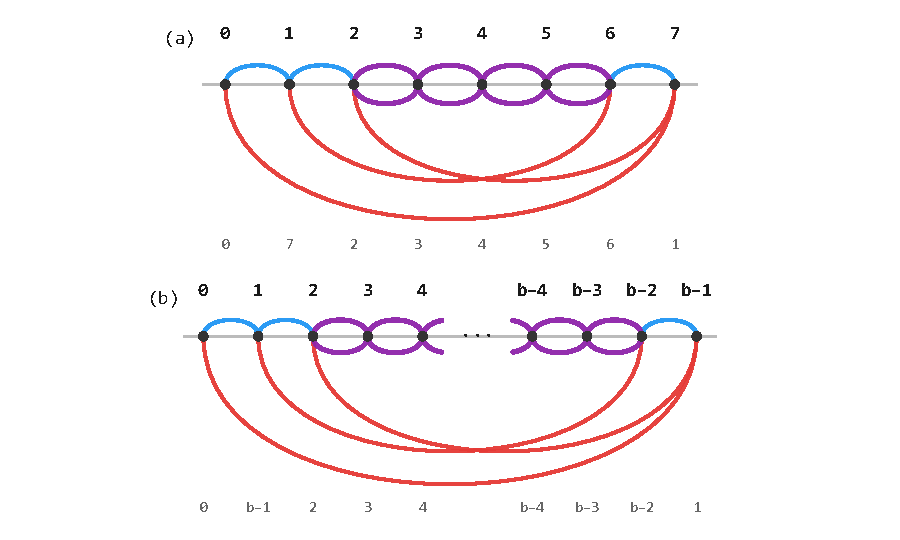
\includegraphics[width=.92\textwidth]{assets/fig_gadget_Tb.pdf}
\caption{The gadget $H_{T_b}$: (a) the instance $T_8 = (0,7,2,3,4,5,6,1)$;
(b) general even $b$, the middle of the segment elided. Vertices are positions on a
line, with the value $T_b(i)$ in small gray below; blue arcs above the line are
P-edges, red arcs below are V-edges, and a purple pair of mirrored arcs is a doubled
pair. The doubled run on the segment $S = \{2,\dots,b{-}2\}$ is flanked by the three
P-only edges $\{0,1\}, \{1,2\}, \{b{-}2,b{-}1\}$ and the three V-only edges
$\{0,b{-}1\}, \{2,b{-}1\}, \{1,b{-}2\}$; the terminals are $0$ ($= p_0 = v_0$),
$1$ ($= v_1$), and $b{-}1$ ($= p_1$).}
\label{fig:Tb}
\end{figure}

\begin{lemma}[Segment behavior]\label{lem:segment}
Let $Q$ be a PC path in $H_{T_b}$.
\begin{enumerate}
\item[(a)] While inside $S$, $Q$ moves monotonically in position (each interior vertex
of $S$ is adjacent only to its two position-neighbors), and $Q$ can leave $S$ only from
vertex $2$ or vertex $b-2$.
\item[(b)] Suppose $Q$ enters $S$ at one end ($2$ or $b-2$) by an edge of color $c$, at
a moment when no vertex of $S$ has yet been visited, and later leaves $S$. Then either
it leaves immediately from the entry vertex (using the other external edge there, of
color $\bar c$), or it traverses all of $S$ to the far end; in the latter case its
$b-4$ internal edges alternate colors starting with $\bar c$, so (since $b$ is even,
making $b - 4$ even) the last internal edge has color $c$, and any edge by which $Q$
then leaves $S$ has color $\bar c$.
\end{enumerate}
\end{lemma}

\begin{proof}
(a) is immediate from the inventory: a simple path cannot reverse inside a path graph.
For (b): leaving from the entry vertex means the run in $S$ is that single vertex; the
two external edges at $2$ (resp.\ $b-2$) have different colors, and the PC condition
forces the exit edge to differ from the entry edge, i.e.\ to be the other one, of color
$\bar c$. Otherwise the run proceeds monotonically and exits only at the far end,
having covered all of $S$ with internal edges $g_1,\dots,g_{b-4}$. The PC condition at
the entry vertex gives $g_1 = \bar c$ (both colors are available on every doubled pair;
the PC condition forces the alternation), alternation gives $g_m=\bar c$ for odd $m$
and $g_m=c$ for even $m$, and $b-4$ is even, so $g_{b-4}=c$; the PC condition at the far
end forces the exit edge to have color $\ne c$.
\end{proof}

\subsection{The classification theorem}

\begin{theorem}[Classification of admissible visits]\label{thm:classification}
Let $b \ge 6$ be even. Up to the reversal symmetry of Lemma~\ref{lem:reversal},
the graph $H_{T_b}$ has exactly five admissible visits. They are the following, each with the role pair shown:
\begin{center}
\begin{tabular}{clll}
\toprule
 & vertices & edges (colors) & role pair \\
\midrule
(V1) & $0$ & --- & $\{p_0, v_0\}$ \\
(V2) & $0,\ b-1$ & $\mathrm V\{0,b{-}1\}$ & $\{p_0, p_1\}$ \\
(V3) & $0,\ 1$ & $\mathrm P\{0,1\}$ & $\{v_0, v_1\}$ \\
(V4) & $b-1,\ 0,\ 1$ & $\mathrm V\{0,b{-}1\},\ \mathrm P\{0,1\}$ & $\{p_1, v_1\}$ \\
(V5) & $b-1,\ 2,\ 1$ & $\mathrm V\{2,b{-}1\},\ \mathrm P\{1,2\}$ & $\{p_1, v_1\}$ \\
\bottomrule
\end{tabular}
\end{center}
In particular: the role pairs $\{p_0, v_1\}$ and $\{v_0, p_1\}$ admit no visit; the
only visit for $\{p_0, p_1\}$ is (V2); the only visit for $\{v_0, v_1\}$ is (V3); and
$M(T_b) = 3$.
\end{theorem}

\begin{proof}
That each listed visit is admissible is a direct check from Lemma~\ref{lem:inventory}.
(V1): vertex $0$ carries $p_0$ and $v_0$ with different port colors. (V2): first
$=$ last edge $\mathrm V \ne \pc(p_0) = \pc(p_1) = \mathrm P$. (V3): first $=$ last edge
$\mathrm P \ne \pc(v_0) = \pc(v_1) = \mathrm V$. (V4), (V5): first edge $\mathrm V \ne
\pc(p_1)$, last edge $\mathrm P \ne \pc(v_1)$, and the middle vertex alternates the
colors. The role pairs are forced: e.g.\ in (V2) the first edge is $\mathrm V$, so the
role at $0$ has port color $\ne \mathrm V$, i.e.\ $p_0$; the same one-line check fixes
each role pair.

It remains to show no other admissible visit exists. Type-(ii) visits need a vertex
carrying two roles of different port colors; by Lemma~\ref{lem:inventory} the only such
vertex is $0 = p_0 = v_0$, giving (V1). A type-(i) visit starts at a terminal vertex
with a constrained first color (Lemma~\ref{lem:reversal}(b)). The terminal vertices are
$0, 1, b-1$, giving exactly four (start vertex, first color) \emph{stems}:
\[
\text{(A) } (0, \mathrm V) \text{ [role } p_0\text{]}, \quad
\text{(B) } (0, \mathrm P) \text{ [role } v_0\text{]}, \quad
\text{(C) } (1, \mathrm P) \text{ [role } v_1\text{]}, \quad
\text{(D) } (b-1, \mathrm V) \text{ [role } p_1\text{]}.
\]
Every admissible visit, read from its first vertex, extends one of these stems, so it
suffices to enumerate, for each stem, every PC continuation, recording the moments at
which the path stands at a terminal vertex with a last-edge color admissible for a role
there. We use the \emph{forcing facts} from Lemma~\ref{lem:inventory}:
(F1) vertex $0$ has exactly one P-edge ($\{0,1\}$) and one V-edge ($\{0,b-1\}$);
(F2) vertex $1$ has exactly one V-edge ($\{1,b-2\}$);
(F3) vertex $b-1$ has exactly one P-edge ($\{b-2,b-1\}$);
plus the segment behavior of Lemma~\ref{lem:segment}. No vertex of $S$ is a terminal,
so a path stranded in $S$ can never end an admissible visit there.

\medskip
\noindent\textbf{Stem (A): start $0$, first edge $\mathrm V$.}
By (F1) the first edge is $\mathrm V\{0, b-1\}$; the path stands at $b-1$, last color
$\mathrm V$. \emph{Record:} role $p_1$ at $b-1$ has $\pc = \mathrm P \ne \mathrm V$, so
$(0, b-1)$ is admissible: this is (V2). Continue: next $\ne \mathrm V$, so by (F3)
$\mathrm P\{b-2,b-1\}$; enter $S$ at $b-2$, entry color $\mathrm P$, $S$ untouched. By
Lemma~\ref{lem:segment}(b):
\begin{itemize}
\item \emph{Immediate exit at $b-2$} by $\mathrm V\{1, b-2\}$: stand at $1$, last color
$\mathrm V$; the only role at $1$ is $v_1$ ($\pc = \mathrm V$): not admissible.
Continue from $1$: next $\ne \mathrm V$, so a P-edge; $\{0,1\}$ excluded ($0$ visited),
leaving $\mathrm P\{1,2\}$ into $S$ at $2$. From $2$, next $\ne \mathrm P$:
$\mathrm V\{2,b-1\}$ excluded ($b-1$ visited), leaving the V-side of $\{2,3\}$; from $3$
the path moves monotonically up and strands (exits are $2$, behind it, and $b-2$,
visited). No admissible visit.
\item \emph{Full crossing to $2$}: arrival at $2$ by color $\mathrm P$
(Lemma~\ref{lem:segment}(b) with $c=\mathrm P$); exit must be $\mathrm V$; the only
V-external edge at $2$ is $\{2,b-1\}$ with $b-1$ visited. Strands. No admissible visit.
\end{itemize}
\emph{Stem (A) yields exactly (V2).}

\medskip
\noindent\textbf{Stem (B): start $0$, first edge $\mathrm P$.}
By (F1) the first edge is $\mathrm P\{0,1\}$; stand at $1$, last color $\mathrm P$.
\emph{Record:} role $v_1$ at $1$ has $\pc = \mathrm V \ne \mathrm P$: admissible: (V3).
Continue: next $\ne \mathrm P$, so by (F2) $\mathrm V\{1, b-2\}$; enter $S$ at $b-2$,
entry color $\mathrm V$, $S$ untouched. By Lemma~\ref{lem:segment}(b):
\begin{itemize}
\item \emph{Immediate exit at $b-2$} by $\mathrm P\{b-2, b-1\}$: stand at $b-1$, last
color $\mathrm P$; the only role at $b-1$ is $p_1$ ($\pc=\mathrm P$): not admissible.
Continue from $b-1$: next $\ne \mathrm P$, so a V-edge; $\{0,b-1\}$ excluded ($0$
visited), leaving $\mathrm V\{2,b-1\}$ into $S$ at $2$. From $2$, next $\ne \mathrm V$:
$\mathrm P\{1,2\}$ excluded ($1$ visited), leaving the P-side of $\{2,3\}$; monotone up
and strands ($b-2$ visited). No admissible visit.
\item \emph{Full crossing to $2$}: arrival color $\mathrm V$; exit must be $\mathrm P$;
only P-external edge at $2$ is $\{1,2\}$, and $1$ is visited. Strands. No admissible
visit.
\end{itemize}
\emph{Stem (B) yields exactly (V3).}

\medskip
\noindent\textbf{Stem (C): start $1$, first edge $\mathrm P$.}
The P-edges at $1$ are $\{0,1\}$ and $\{1,2\}$; two branches.
\begin{itemize}
\item \emph{Branch $1 \to 0$.} At $0$, last color $\mathrm P$. \emph{Record:} $v_0$
($\pc=\mathrm V$) admissible: (V3) reversed. Continue: next $\ne \mathrm P$, by (F1)
$\mathrm V\{0, b-1\}$; at $b-1$, last color $\mathrm V$. \emph{Record:} $p_1$
admissible: (V4) reversed. Continue: next $\ne \mathrm V$, by (F3) $\mathrm P\{b-2,b-1\}$
into $S$ at $b-2$, entry color $\mathrm P$, $S$ untouched. Immediate exit by
$\mathrm V\{1,b-2\}$: $1$ visited. Full crossing: arrival at $2$ color $\mathrm P$, exit
must be $\mathrm V$: only $\{2,b-1\}$, visited. Strands; branch closed.
\item \emph{Branch $1 \to 2$.} Enter $S$ at $2$ by $\mathrm P\{1,2\}$, entry color
$\mathrm P$, $S$ untouched. Immediate exit by $\mathrm V\{2, b-1\}$: at $b-1$, last
color $\mathrm V$. \emph{Record:} $p_1$ admissible: (V5) reversed. Continue from $b-1$:
next $\ne \mathrm V$, by (F3) $\mathrm P\{b-2,b-1\}$ into $S$ at $b-2$ -- but $S$ is now
touched (vertex $2$): from $b-2$ the non-$\mathrm P$ continuations are
$\mathrm V\{1,b-2\}$ ($1$ visited) and the V-side of $\{b-3,b-2\}$, after which the path
moves monotonically down and strands at $3$ ($2$ visited). Branch closed.
Alternatively, full crossing $2 \to b-2$ with entry color $\mathrm P$ arrives at $b-2$
by color $\mathrm P$; exit must be $\mathrm V$: only $\{1, b-2\}$, $1$ visited. Strands;
branch closed.
\end{itemize}
\emph{Stem (C) yields exactly (V3), (V4), (V5) (reversed).}

\medskip
\noindent\textbf{Stem (D): start $b-1$, first edge $\mathrm V$.}
The V-edges at $b-1$ are $\{0, b-1\}$ and $\{2, b-1\}$; two branches.
\begin{itemize}
\item \emph{Branch $b-1 \to 0$.} At $0$, last color $\mathrm V$. \emph{Record:} $p_0$
admissible: (V2) reversed. Continue: next $\ne \mathrm V$, by (F1) $\mathrm P\{0,1\}$;
at $1$, last color $\mathrm P$. \emph{Record:} $v_1$ admissible: (V4). Continue: next
$\ne \mathrm P$, by (F2) $\mathrm V\{1,b-2\}$ into $S$ at $b-2$, entry color $\mathrm V$,
$S$ untouched. Immediate exit by $\mathrm P\{b-2,b-1\}$: $b-1$ visited. Full crossing:
arrival at $2$ color $\mathrm V$, exit must be $\mathrm P$: only $\{1,2\}$, $1$ visited.
Strands; branch closed.
\item \emph{Branch $b-1 \to 2$.} Enter $S$ at $2$ by $\mathrm V\{2,b-1\}$, entry color
$\mathrm V$, $S$ untouched. Immediate exit by $\mathrm P\{1,2\}$: at $1$, last color
$\mathrm P$. \emph{Record:} $v_1$ admissible: (V5). Continue from $1$: next
$\ne \mathrm P$, by (F2) $\mathrm V\{1,b-2\}$ into $S$ at $b-2$ -- $S$ touched (vertex
$2$): from $b-2$ the non-$\mathrm V$ continuations are $\mathrm P\{b-2,b-1\}$ ($b-1$
visited) and the P-side of $\{b-3,b-2\}$, then monotone descent stranding at $3$ ($2$
visited). Branch closed. Alternatively, full crossing $2 \to b-2$ with entry color
$\mathrm V$ arrives by color $\mathrm V$; exit must be $\mathrm P$: only $\{b-2,b-1\}$,
$b-1$ visited. Strands; branch closed.
\end{itemize}
\emph{Stem (D) yields exactly (V2), (V4), (V5).}

\medskip
Collecting the four stems: every admissible visit is one of (V1)--(V5) up to reversal,
each realized only with the listed role pair (checked at each \emph{Record} step). No
admissible visit realizes $\{p_0, v_1\}$ or $\{v_0, p_1\}$, and the maximum size is
$3$, attained by (V4) and (V5).
\end{proof}

\begin{corollary}\label{cor:M3}
$M(T_b) = 3$ for every even $b \ge 6$, and $c^* := \liminf_n \pmin(n)/n$ satisfies
$c^* \le 6/b$ for every even $b \ge 6$; hence $c^* = 0$.
\end{corollary}

\begin{proof}
$M(T_b) = 3$ is part of Theorem~\ref{thm:classification}. Taking $\pi_i = T_b$ for all
$i$ in Theorem~\ref{thm:inflation} and letting $a \to \infty$:
$\pmin(ab)/(ab) \le \bigl((2a-3)\cdot 3 + 2b\bigr)/(ab) \to 6/b$.
\end{proof}

\begin{remark}[The parity is essential]\label{rem:parity}
For \emph{odd} $b$, $b - 4$ is odd, so the last internal edge of a full crossing has
color $\bar c$ and the exit edge may have color $c$. The route
$0 \xrightarrow{\mathrm P} 1 \xrightarrow{\mathrm V} b-2 \rightsquigarrow 2
\xrightarrow{\mathrm V\{2,b-1\}} b-1$ (full crossing in the middle) then becomes
properly colored, an admissible visit for $\{v_0, p_1\}$ of size $b$.
%% [E20 2026-07-29] Brute-force-confirmation sentence cut (rem:parity); the
%% structural route above already yields M(T_b)=b for odd b.
\end{remark}

A sibling gadget $T'_b$ -- the identity with the values $2$ and $b{-}1$ exchanged --
serves \emph{odd} $b$ by the same mechanism with the good parity reversed; its
admissible visits are classified completely in Appendix~\ref{app:oddb}, and it enters
the transit-floor bound through Proposition~\ref{prop:floor-upper}.

\begin{corollary}[Two visits to one $T_b$-block]\label{cor:pairs}
Let $\sigma = \tau[\pi_1, \dots, \pi_a]$ be an inflation, $B_i$ a block whose pattern
$\pi_i$ equals $T_b$ for some even $b \ge 6$, and $Q$ a PC path in $H_\sigma$. Then the
interior visits of $Q$ to $B_i$ have total size at most $4$.
\end{corollary}

\begin{proof}
By Lemma~\ref{lem:crosscount}, $B_i$ has at most four incident cross edges, one per
role; each interior visit uses two distinct ones (entry and exit), and every cross edge
is used at most once. Hence there are at most two interior visits; if at most one, its
size is at most $M(T_b)=3\le4$. If two, they use all four cross edges, so their role
pairs partition $\{p_0, p_1, v_0, v_1\}$, and they are vertex-disjoint (disjoint runs of
the simple path $Q$). By Theorem~\ref{thm:classification} the three partitions give:
\begin{itemize}
\item $\{p_0, p_1\}/\{v_0, v_1\}$: the only visits are (V2)$=(0,b-1)$ and (V3)$=(0,1)$,
which share vertex $0$ -- impossible;
\item $\{p_0, v_1\}/\{v_0, p_1\}$: no visits exist for either pair -- impossible;
\item $\{p_0, v_0\}/\{p_1, v_1\}$: the $\{p_0,v_0\}$ visit is (V1) at vertex $0$, and
the $\{p_1,v_1\}$ visit is (V4) or (V5); since (V4)$=(b-1,0,1)$ contains vertex $0$ it
cannot be disjoint from (V1), so the disjoint pair is (V1) with (V5), of sizes $1$ and
$3$: total $4$. (In every case the total is at most $4$.)
\end{itemize}
\end{proof}

\section{Proof of the main theorem}\label{sec:main}

We prove the bound advertised in Theorem~\ref{thm:main-intro}. The family is
$\sigma_{a,b} = \mathrm{id}_a[T_b, \dots, T_b]$, i.e.\ $\sigma_{a,b}(jb+r) = jb + T_b(r)$,
and the proof combines the two-visit bound for one $T_b$-block
(Corollary~\ref{cor:pairs}) with the inflation count of Section~\ref{sec:inflation}.

%% [E20 2026-07-29] thm:main reduced to the family bound; the pmin(n) half is now
%% the proof of Theorem 1.1 directly, so the main theorem carries one number.
\begin{theorem}[Family bound]\label{thm:main}
For every even $b \ge 6$ and $a \ge 2$, $\ \rho(\sigma_{a,b}) \le 4a + 2b$.
\end{theorem}

\begin{proof}
Let $Q$ be a PC path in $H_{\sigma_{a,b}}$ with $q$ visits. If
$q = 1$ then $|Q| \le b$. Otherwise, by Lemma~\ref{lem:visits} the first and last visits
have at most $b$ vertices each, and by Corollary~\ref{cor:pairs} the interior visits
contribute at most $4$ per block, i.e.\ at most $4a$ in total. Hence
$\rho(\sigma_{a,b}) \le 4a + 2b$.
\end{proof}

\begin{proof}[Proof of Theorem~\ref{thm:main-intro}]
Let $b = 2\lfloor \sqrt n / 2 \rfloor$, so $b$ is even,
$\sqrt n - 2 < b \le \sqrt n$, and $b \ge 10$ since $n \ge 100$. Let
$a = \lfloor n/b \rfloor \ge 2$ and $s = n - (a-1)b$, so $b \le s < 2b$. Define
$\sigma \in S_n$ as the inflation (identity outer permutation) of:
\begin{itemize}
\item if $s$ even: $a - 1$ copies of $T_b$ and one copy of $T_s$ ($s$ even,
$s \ge b \ge 10$);
\item if $s$ odd: $a - 1$ copies of $T_b$, one copy of $T_{s-3}$, and one block of size
$3$ with identity pattern $\iota_3 = (0,1,2)$ ($s-3$ even, $s-3 \ge b-2 \ge 8$, since
$s$ odd and $b$ even force $s \ge b+1$).
\end{itemize}
The number of blocks is at most $a+1 \le n/b + 1$, and each block is one of $T_b$, $T_s$,
$T_{s-3}$, or $\iota_3$. Interior visits contribute at most $4$ per $T$-block
(Corollary~\ref{cor:pairs}, which applies verbatim to $T_b$, $T_s$, $T_{s-3}$) and at
most $2 \cdot 3 = 6$ for the single $\iota_3$-block (at most two interior visits, by
Lemma~\ref{lem:crosscount}, of size at most $3$ each). The two end visits contribute at
most $2(2b-1)$, since the largest block has size at most $2b-1$. Hence
\[
\pmin(n) \;\le\; 4\Bigl(\frac n b + 1\Bigr) + 6 + 2(2b-1) \;=\; \frac{4n}{b} + 4b + 8
\;\le\; \bigl(4\sqrt n + 10\bigr) + 4\sqrt n + 8 \;\le\; 8\sqrt n + 20,
\]
using $4n/(\sqrt n - 2) = 4\sqrt n + 8\sqrt n/(\sqrt n - 2) \le 4\sqrt n + 10$ for
$\sqrt n \ge 10$.
\end{proof}

\begin{remark}[A weaker bound without the full classification]\label{rem:crude}
If one uses only the value $M(T_b) = 3$ and not the two-visit refinement, the Inflation
Lemma (Theorem~\ref{thm:inflation}) already gives $\rho(\sigma_{a,b}) \le 6a + 2b$ and,
by the same choice of blocks (each of transit number at most $3$),
$\pmin(n) \le (2m-3)\cdot 3 + 2(2b-1) \le 6n/b + 4b - 5 \le 10\sqrt n + 10$ for
$n \ge 100$. The refinement to $8\sqrt n + 20$ is what the two-visit corollary buys.
\end{remark}

\begin{proposition}[Explicit long path: the family is $\Theta(a+b)$]\label{prop:lower}
For every even $b \ge 6$ and $a \ge 2$, $\ \rho(\sigma_{a,b}) \ge 2a + 2b - 7$.
\end{proposition}

\begin{proof}
Write $(j, \ell)$ for the vertex at position $jb + \ell$ ($0 \le j < a$,
$0 \le \ell < b$), so block $j$ is a copy of $H_{T_b}$ on $\{(j,0), \dots, (j,b-1)\}$,
with values $(j,0) \mapsto jb$, $(j,1) \mapsto jb + b - 1$, $(j,\ell) \mapsto jb + \ell$
for $2 \le \ell \le b-2$, and $(j, b-1) \mapsto jb + 1$. Besides the internal edges
(Lemma~\ref{lem:inventory} in each block), the cross edges are the P-edges
$\{(j, b-1), (j+1, 0)\}$ and the V-edges $\{(j, 1), (j+1, 0)\}$. Within block $j$ note
the V-edges $\{(j,0), (j,b-1)\}$ and $\{(j,2), (j,b-1)\}$.

The following walk is a PC path; colors are indicated over each step, and each edge
exists by the inventory.
\begin{itemize}
\item \emph{Stage 1 (block $0$).} Start at $(0, b-2)$ and descend the segment to
$(0, 2)$ along the doubled run, choosing colors $\mathrm V, \mathrm P, \mathrm V, \dots$;
this uses $b - 4$ edges, and since $b - 4$ is even the last (into $(0,2)$) has color
$\mathrm P$. Then take $\mathrm V\,\{(0,2), (0,b-1)\}$, then the P-cross edge to
$(1, 0)$.
\item \emph{Stage 2 (blocks $1, \dots, a-2$).} From $(j, 0)$ (entered by a P-cross
edge) take $\mathrm V\,\{(j,0), (j,b-1)\}$, then the P-cross edge to $(j+1, 0)$; repeat.
\item \emph{Stage 3 (block $a-1$).} From $(a-1, 0)$ (entered by a P-cross edge) take
$\mathrm V\,\{(a-1,0), (a-1,b-1)\}$, then $\mathrm P\,\{(a-1,b-2), (a-1,b-1)\}$, then
descend the segment from $(a-1, b-2)$ to $(a-1, 2)$ choosing colors
$\mathrm V, \mathrm P, \dots$, stopping at $(a-1, 2)$.
\end{itemize}
All vertices are distinct (stages use disjoint blocks; within a stage the listed
vertices are distinct), and consecutive edge colors differ at every junction. The vertex
count is $(b - 2)$ in stage 1 ($b-3$ segment vertices plus $(0, b-1)$), $2(a-2)$ in
stage 2, and $(b - 1)$ in stage 3 ($(a-1,0)$, $(a-1,b-1)$, and the $b-3$ segment
vertices), totalling $2a + 2b - 7$.
%% [E20 2026-07-29] F2 cut: mechanical-check sentence removed (proof is complete
%% without it; the sec:comp item is E19's call).
\end{proof}

\begin{remark}[Constants; exact values]\label{rem:constants}
Together, Theorem~\ref{thm:main} and Proposition~\ref{prop:lower} give
$2(a+b) - 7 \le \rho(\sigma_{a,b}) \le 4a + 2b$: the family is $\Theta(a + b)$, and with
$a \asymp b$ realizes $\Theta(\sqrt n)$, so the upper bound of
Theorem~\ref{thm:main-intro} is achieved by this family up to the constant. Exact
machine computation (Appendix~\ref{sec:comp}) gives $\rho(\sigma_{a,b}) = 2a + 2b - 4$ at
every tested point up to $n = 720$; we conjecture this holds for all $a \ge 3$, even
$b \ge 6$, but we neither prove nor use it. Optimizing the proven upper bound $4a + 2b$
at $n = ab$ with $b \asymp \sqrt{2n}$ gives $\pmin(n) \le 4\sqrt{2n} + O(1) \approx
5.66\sqrt n$ along such $n$.
\end{remark}

\section{The transit floor: no pattern has transit number below three}
\label{sec:floor}

The main theorem rests on patterns whose transit number is $3$ while their size grows.
Within the inflation calculus, one parameter is decisive: how small the transit number
of a pattern can be made. Define
\[
  \mu(b) \;:=\; \min_{\pi \in S_b} M(\pi) \qquad (b \ge 2).
\]
Any family of patterns with $\mu$-optimal transit numbers gives the best interior-visit
bookkeeping the Inflation Lemma can produce. This section determines $\mu$ completely.

\begin{theorem}[Transit floor]\label{thm:floor}
$\mu(b) = 3$ for every $b \ge 3$. (For $b = 2$, both permutations have $M = 2$, so
$\mu(2) = 2$.)
\end{theorem}

The upper bound is a construction, the lower bound a structure theorem; we prove them
in turn. Together they say the gadgets of this paper are optimal in the transit
parameter: no choice of inflation blocks can beat $M = 3$ at any size.

\subsection{The upper bound: gadgets at every size}

\begin{proposition}\label{prop:floor-upper}
$\mu(b) \le 3$ for every $b \ge 3$.
\end{proposition}

\begin{proof}
For $b = 3$ the inequality is trivial: an admissible visit has at most $b$ vertices,
so $M(\pi) \le 3$ for every $\pi \in S_3$. For even $b \ge 6$,
Corollary~\ref{cor:M3} gives $M(T_b) = 3$. For odd $b \ge 7$, let
\[
  T'_b \;=\; (0,\ 1,\ b{-}1,\ 3,\ 4,\ \dots,\ b{-}2,\ 2) \in S_b
\]
be the identity with the values $2$ and $b-1$ exchanged -- a sibling of $T_b$, which
exchanges $1$ and $b-1$. Appendix~\ref{app:oddb} classifies the admissible visits of
$H_{T'_b}$ completely, in the manner of Theorem~\ref{thm:classification}: up to
reversal there are exactly five, of sizes $1, 3, 3, 3, 3$, so $M(T'_b) = 3$. (The
parity mechanism is the same doubled-run obstruction as in
Lemma~\ref{lem:segment}, with the run shortened by one vertex, which is exactly what
reverses the good parity from even $b$ to odd $b$.) The two remaining sizes $b = 4, 5$
are settled by the exhaustive enumeration already reported in
Appendix~\ref{sec:comp}: $\min_{\pi \in S_b} M(\pi) = 3$ for $4 \le b \le 9$; for $b=5$
the pattern $T'_5 = (0,1,4,3,2)$ attains it, with admissible-visit list
$(0)$, $(0,1,2)$, $(0,1,4)$, $(2,1,4)$, $(2,3,4)$.
\end{proof}

\subsection{The lower bound: every pattern admits a visit of size three}

The lower bound cannot be proved by a local or greedy argument: for the identity
permutation the \emph{smallest} witness visit produced below is a
terminal-to-terminal path through all $b$ vertices, so no argument that exhibits a
bounded-size certificate can succeed uniformly. The proof instead builds the witness
globally, from one matching inside each color class. Three elementary lemmas about
matchings in paths do all the work. Throughout, $\pi \in S_b$ with $b \ge 3$; the
\emph{P-path} is the Hamiltonian path $0 - 1 - \cdots - (b-1)$ of P-edges and the
\emph{V-path} is the Hamiltonian path $\inv\pi(0) - \inv\pi(1) - \cdots - \inv\pi(b-1)$
of V-edges. For a matching $M$ contained in one of these paths, we say $M$
\emph{exposes} the vertices it does not cover.

\begin{lemma}[Matching unions]\label{lem:munion}
Let $M_P$ be a matching contained in the P-edges and $M_V$ a matching contained in the
V-edges, and let $U$ be their union, keeping colors (if a doubled pair contributes an
edge to each, $U$ retains both parallel edges). Then:
\begin{enumerate}
\item[(a)] every vertex has degree $\le 2$ in $U$; more precisely, the degree of $x$
in $U$ equals the number of the two matchings that cover $x$;
\item[(b)] the connected components of $U$ are simple paths (possibly single vertices)
and cycles, and along any component the edges alternate between $M_P$ and $M_V$, hence
alternate colors: every component is properly colored;
\item[(c)] the degree-$1$ vertices are exactly those covered by exactly one of the two
matchings, and the unique $U$-edge at such a vertex belongs to the matching covering
it. If $U$ has exactly $2\ell$ vertices of degree $1$, then $U$ has exactly $\ell$
components that are paths with at least one edge, their ends pairing up the degree-$1$
vertices.
\end{enumerate}
\end{lemma}

\begin{proof}
(a) Each matching contributes at most one edge per vertex. Consecutive edges of a walk
in $U$ share a vertex, so they cannot lie in the same matching; hence they alternate
between $M_P$ and $M_V$, and since $M_P$-edges are P-colored and $M_V$-edges V-colored,
the colors alternate, giving (b) (maximum degree $2$ makes every component a path or a
cycle; a doubled pair with both copies in $U$ is a $2$-cycle component). The ends of the
path components are the vertices of degree $\le 1$, giving (c).
\end{proof}

\begin{lemma}[Prescribed exposure]\label{lem:expose}
Let $Q = x_0 - x_1 - \cdots - x_{m-1}$ be a path and let
$S \subseteq \{x_0,\dots,x_{m-1}\}$.
A matching of $Q$ exposing exactly $S$ exists if and only if every maximal run of
consecutive non-exposed vertices (in path order) has even size. In particular:
\begin{enumerate}
\item[(a)] $m$ odd: a matching exposing exactly $\{x_j\}$ exists iff $j$ is even;
\item[(b)] $m$ even: a perfect matching exists, and a matching exposing exactly
$\{x_i, x_j\}$ ($i < j$) exists iff $i$ is even and $j$ is odd.
\end{enumerate}
\end{lemma}

\begin{proof}
If every run of non-exposed vertices is even, pair each run off consecutively.
Conversely, a matching of a path covering a contiguous run of vertices bounded by
exposed vertices must pair within the run, forcing even size. For (a), the runs have
sizes $j$ and $m-1-j$, both even iff $j$ is even and $m$ is odd; for (b), the runs
have sizes $i$, $j-i-1$, $m-1-j$, all even iff $i$ is even, $j$ is odd, $m$ is even.
\end{proof}

\begin{lemma}[Exposure trick]\label{lem:trick}
Suppose $M_P$ exposes exactly the vertex set $S_P$ within the P-path and $M_V$ exposes
exactly $S_V$ within the V-path, and let $U$ be their union. Then:
\begin{enumerate}
\item[(a)] the degree-$1$ vertices of $U$ are exactly
$(S_P \cup S_V) \setminus (S_P \cap S_V)$; the vertices of $S_P \cap S_V$ are isolated;
all others have degree $2$;
\item[(b)] \emph{(opposite exposure $\Rightarrow$ odd size $\ge 3$)} if a path
component of $U$ has one end $x \in S_P \setminus S_V$ and the other end
$y \in S_V \setminus S_P$, then its end edges are V-colored at $x$ and P-colored at
$y$, its edge count is even, and it has at least $2$ edges: its size is odd and
$\ge 3$;
\item[(c)] \emph{(same exposure $\Rightarrow$ even size $\ge 2$)} if both ends lie in
$S_P \setminus S_V$, the end edges are V-colored at both ends, the edge count is odd,
and the size is even and $\ge 2$, with size exactly $2$ precisely when the two ends are
joined by a single $M_V$-edge (symmetrically with the colors exchanged for two ends in
$S_V \setminus S_P$).
\end{enumerate}
\end{lemma}

\begin{proof}
(a) restates Lemma~\ref{lem:munion}(a). For (b): $x \in S_P \setminus S_V$ is covered
only by $M_V$, so its unique $U$-edge is V-colored; likewise the unique edge at $y$ is
P-colored (Lemma~\ref{lem:munion}(c)). Alternation with first color V and last color P
forces an even number of edges, and the component has at least one edge since its ends
have degree $1$. If it had exactly one edge $e = \{x,y\}$, then $e$, being $x$'s edge,
lies in $M_V$; but then $M_V$ covers $y$, contradicting $y \in S_V$. So the edge count
is even and $\ge 2$, and the size (edges plus one) is odd and $\ge 3$. For (c): both
end edges are V-colored, so alternation $\mathrm V \cdots \mathrm V$ gives an odd edge
count $\ge 1$; the size is even and $\ge 2$, and size $2$ is exactly the single-edge
case, which forces that edge into $M_V$.
\end{proof}

\begin{theorem}[Floor lower bound]\label{thm:floor-lower}
For every $\pi \in S_b$ with $b \ge 3$, the graph $H_\pi$ has a type-(i) admissible
visit of size $\ge 3$. Hence $M(\pi) \ge 3$.
\end{theorem}

\begin{proof}
Write $v_0 = \inv\pi(0)$ and $v_1 = \inv\pi(b-1)$; these are distinct vertices since
$b \ge 2$. All matchings below live inside the P-path or the V-path, and their
existence is by Lemma~\ref{lem:expose}, using the following indices: vertex $0$ has
position-index $0$ and vertex $b-1$ has position-index $b-1$ in the P-path; $v_0$ has
value-index $0$ and $v_1$ has value-index $b-1$ in the V-path.

\medskip
\noindent\textbf{Case 1: $b$ odd.}
Both P-path indices $0, b-1$ and both V-path indices $0, b-1$ are even. Set
$c := v_1$ if $v_1 \ne 0$, and otherwise $c := v_0$; in the latter case
$\pi(0) = b-1 \ne 0$, so $v_0 = \inv\pi(0) \ne 0$. Either way $c \ne 0$, and $c$ has
V-path index $0$ or $b-1$, both even. By Lemma~\ref{lem:expose}(a) choose $M_P$
exposing exactly $\{0\}$ (concretely $\{1,2\},\{3,4\},\dots,\{b-2,b-1\}$) and $M_V$
exposing exactly $\{c\}$. Then $S_P = \{0\}$ and $S_V = \{c\}$ are disjoint, so by
Lemma~\ref{lem:trick}(a) the union $U$ has exactly two degree-$1$ vertices, $0$ and
$c$, hence exactly one path component, from $0$ to $c$. By Lemma~\ref{lem:trick}(b) it
is a properly colored path of odd size $\ge 3$ whose first edge is V-colored at vertex
$0$ and whose last edge is P-colored at $c$. Assign the role $p_0$ at vertex $0$ (port
color P $\ne$ V) and the role $v_1$ or $v_0$ at $c$ (port color V $\ne$ P): a type-(i)
admissible visit of size $\ge 3$.

\medskip
\noindent\textbf{Case 2: $b$ even and $\{\pi(0), \pi(b-1)\} \ne \{2k, 2k+1\}$ for
every $k$.}
By Lemma~\ref{lem:expose}(b) choose $M_V$ to be the perfect matching of the V-path
(value pairs $(0,1), (2,3), \dots, (b-2,b-1)$) and $M_P$ exposing exactly
$\{0, b-1\}$ (indices $0$ even and $b-1$ odd). Then $S_P = \{0, b-1\}$, $S_V =
\emptyset$: the union has exactly one path component, from $0$ to $b-1$, with V-colored
end edges at both ends, of even size $\ge 2$ (Lemma~\ref{lem:trick}(c)). Size $2$ would
mean the single edge $\{0, b-1\} \in M_V$, i.e.\ $\{\pi(0), \pi(b-1)\}$ is one of the
value pairs $\{2k, 2k+1\}$ -- excluded by hypothesis. So the size is even and
$\ge 4$; with roles $p_0, p_1$ (port colors P, end edges V) this is a type-(i)
admissible visit of size $\ge 4$.

\medskip
\noindent\textbf{Case 3: $b$ even and $\{\pi(0), \pi(b-1)\} = \{2k, 2k+1\}$ for some
$k$.}
By Lemma~\ref{lem:expose}(b) choose $M_P$ exposing exactly $\{0, b-1\}$ and $M_V$
exposing exactly $\{v_0, v_1\}$ (value-indices $0$ even and $b-1$ odd; the exposed
value pairs are $(1,2), (3,4), \dots, (b-3,b-2)$). Consider the coincidence set
$T := \{0, b-1\} \cap \{v_0, v_1\}$.

\emph{Case 3a: $T = \emptyset$.} There are four degree-$1$ vertices
$0, b-1, v_0, v_1$, hence exactly two path components pairing them up. If some
component joins a P-terminal to a V-terminal, Lemma~\ref{lem:trick}(b) makes it an
admissible visit of odd size $\ge 3$ (roles with opposite port colors at its ends) ---
done. Otherwise one component joins $0$ to $b-1$ and the other joins $v_0$ to $v_1$,
both of even size $\ge 2$ (Lemma~\ref{lem:trick}(c)). If the $0 \leadsto b-1$
component had size $2$, then $\{0,b-1\} \in M_V$, so $\{\pi(0), \pi(b-1)\}$ would be
one of the value pairs $\{2j+1, 2j+2\}$ -- an odd-aligned consecutive pair -- while
the case hypothesis makes it even-aligned; a two-element set of consecutive integers
cannot be both. So that component has even size $\ge 4$, and with roles $p_0, p_1$ it
is an admissible visit of size $\ge 4$ -- done.

\emph{Case 3b: $|T| = 1$.} Let $t$ be the coincident vertex ($t \in S_P \cap S_V$ is
isolated in $U$), $x$ the other P-terminal and $y$ the other V-terminal; $x \ne y$
(else $|T| = 2$). The degree-$1$ vertices are exactly $x$ and $y$, so $U$ has one path
component, from $x$ to $y$, which by Lemma~\ref{lem:trick}(b) is an admissible visit of
odd size $\ge 3$ (a P-role at $x$ with V-colored end edge, a V-role at $y$ with
P-colored end edge) -- done.

\emph{Case 3c: $|T| = 2$.} Then $\{v_0, v_1\} = \{0, b-1\}$, i.e.\
$\{\pi(0), \pi(b-1)\} = \{0, b-1\}$, which is a set of consecutive integers only if
$b = 2$ -- contradicting $b \ge 4$ in the presence of the case-3 hypothesis. So this
sub-case is vacuous.

\medskip
Cases 1--3 cover all $\pi \in S_b$, $b \ge 3$.
\end{proof}

\begin{remark}[The witness is necessarily global]\label{rem:global}
For $\pi = \mathrm{id}_b$ with $b$ odd, Case 1 produces the full alternating path
$0 - 1 - \cdots - (b-1)$: the witness has size $b$, not size $3$. This is forced, not
an artifact: in $H_{\mathrm{id}_b}$ every admissible visit joining terminals at the two
ends must traverse the whole doubled path. A proof of Theorem~\ref{thm:floor-lower}
that exhibits a bounded-radius certificate around a terminal therefore cannot exist,
which is why the matching-union construction, whose witness is a \emph{component of a
globally defined graph}, is the right tool.
\end{remark}

\begin{proof}[Proof of Theorem~\ref{thm:floor}]
Combine Proposition~\ref{prop:floor-upper} and Theorem~\ref{thm:floor-lower}; for
$b = 2$, enumerate directly (each of the two patterns admits a size-$2$ visit between
its two P-roles or V-roles, and size $3$ is impossible on $2$ vertices).
\end{proof}

\begin{remark}[Consequences for the method]\label{rem:floor-consequences}
Theorem~\ref{thm:floor} answers the calibration question raised in
Section~\ref{sec:disc}: transit numbers cannot be pushed below $3$, so within the
inflation framework the per-visit cost of this paper's gadgets is optimal, and
improvements to Theorem~\ref{thm:main-intro} must come from the visit \emph{count} or
from outside the inflation method.
%% [E25 cut 2026-07-30] Validation sentence removed (retires E20 flag F3, paired
%% with the sec:comp floor-construction item cut).
\end{remark}

\begin{remark}[The spectrum of transit numbers; data]\label{rem:spectrum}
Exhaustive computation of $\{M(\pi) : \pi \in S_b\}$ for $b \le 8$
(Appendix~\ref{sec:comp}) shows that the attained set is $\{3, 4, \dots, b\}$ for even
$b$ but $\{3\} \cup \{5, \dots, b\}$ for odd $b$: the value $4$ is not attained at
odd $b \le 8$. The maximum $M(\pi) = b$ is always attained (e.g.\ by the identity). We
record the gap at $4$ as data; we have no proof that it persists for odd $b > 8$.
\end{remark}

%% [E5 cut 2026-07-21] Section 10 (sec:blockfail) removed in full: thm:n14
%% (sigma-dagger threshold + S13/S14 censuses), the staircase family (def:stair,
%% lem:stair, lem:stairparity), Chain Collapse (thm:stairchain), No-Block-Floor
%% (thm:noblockfloor), cor:stairconst, rem:extremes. Dangling references remain in
%% the abstract, Sec. 1 (intro par. 4 + best-possible claims), sec:comp anchors,
%% sec:disc, and the appendix closing note -- deferred to the cross-reference pass.

%% [E25 2026-07-30] sec:comp (Computational verification) RELOCATED to the
%% final appendix (after the scrambled ladder); label kept. Ledger: E25.

\section{Lower bounds and open problems}\label{sec:disc}

%% [E14 2026-07-28] Block-bound post-mortem removed (de-historicize); what is
%% known stated positively. b(sigma)'s remaining role: ledger E15.
We work with $\pm1$-blocks (Definition~\ref{def:pmblock}); $b(\sigma)$ is their
number and $\smax(\sigma)$ the largest size. What is known on the lower-bound
side is quickly stated. The only unconditional lower bound we have is the floor
$\rho \ge \smax$ (Proposition~\ref{prop:survive}), and it degenerates exactly
where it is needed most: on permutations whose blocks all have bounded size,
$\smax$ is constant while $n$ grows. Beyond the floor our methods produce no
lower bounds at all, while Theorem~\ref{thm:main-intro} caps everything at
$O(\sqrt n\,)$; we expect the cap to be the truth, i.e.\ that
$\pmin(n) = \Theta(\sqrt n)$. This is the state of the problem we most want
to advertise:

\begin{quote}
\emph{Main open problem. Prove or disprove: $\pmin(n) \to \infty$.}
\end{quote}

The difficulty is easy to underestimate. The graphs $H_\sigma$ are spanning,
connected, of maximum degree four, and every vertex lies on two Hamiltonian
monochromatic paths; the natural intuition is that so much connectivity must force
alternating paths of unbounded length. We know no quantity that makes that
intuition precise. A disproof -- a family with $\rho$ bounded -- would be at least
as interesting, though we do not expect one.
%% [E20 2026-07-29] "warns that small-n exhaustive evidence is weak" sentence cut.

On the gadget side, the calibration question is settled by
Theorem~\ref{thm:floor}: transit numbers cannot be made smaller than $3$ at any size,
so inflation with better blocks cannot improve the method's constants, and
(heuristically) inflation alone cannot beat $\sqrt n$: the end-visit term ties the
bound to the block size, and nesting inflations doubles the visit-count bound per
level. What remains open there is the fine structure of the transit spectrum
(Remark~\ref{rem:spectrum}): is the value $4$ unattained at every odd $b$?

%% [E8 splice 2026-07-28] WP-J Q1/Q2/Q3 (PAPER_SECTION_draft.tex, trimmed: Q4/Q5
%% dropped; Q2 Lovasz-propagation trimmed per E7 -- known bound + provenance now
%% in the scrambled-ladder appendix). The cycles direction is DELETED per E9
%% decision (d). Spliced numbers are campaign-produced; Codex gate audit in
%% flight (P-WPJ.1-.3) -- roll back this splice if it fails. Ledger: E7/E8/E9.

Three further directions, each supported by exact data.

\paragraph{More colors.}
For $k$ permutations $w_1,\dots,w_k$ of a common vertex set, color the edges of
the $k$ Hamiltonian paths $P(w_1),\dots,P(w_k)$ with $k$ colors, one per path,
and let $\pminK{k}(n)$ denote the minimum over all $k$-tuples of the maximum
number of vertices on a properly colored simple path. (For $k=2$ this is
$\pmin(n)$: anchoring one path as the identity is a relabeling.) Adding a color
only adds edges, so
\[
\pmin(n) \;=\; \pminK{2}(n) \;\le\; \pminK{3}(n) \;\le\; \cdots \;\le\; n .
\]
Exhaustive computation (ancillary artifact) gives
$\pminK{3}(n) = n$ for $4 \le n \le 10$: \emph{every} union of three Hamiltonian
paths on at most ten vertices has a properly colored Hamiltonian path -- in
particular a third ordering erases the two-color dips at $n = 7, 8$. But three
orderings do not suffice forever:

\begin{proposition}\label{prop:k3}
$\pminK{3}(11) = 10$. Up to symmetry (permuting the three paths, reversing
paths, and relabeling) there is exactly \emph{one} triple of Hamiltonian paths
on $11$ vertices whose union has no properly colored Hamiltonian path, namely
$w_1 = \mathrm{id}$,
$w_2 = (0,1,2,3,4,6,7,8,5,9,10)$,
$w_3 = (0,1,5,2,3,4,6,7,8,9,10)$
(the identity together with one-step cyclic shifts of the vertex intervals
$[5,8]$ and $[2,5]$); this triple attains $\rho = 10$. The count over anchored
unordered pairs $\{w_2, w_3\}$ is $12$, all in one symmetry orbit.
\end{proposition}

The computation is a census, not a triple-by-triple sweep: a properly colored
path of any two of the three colors survives in the union, so a deficient
triple $(\mathrm{id}, s, t)$ requires all three of its two-color
\emph{shadows} -- the pairs $(\mathrm{id},s)$, $(\mathrm{id},t)$, and
$(s,t) \cong (\mathrm{id}, s^{-1}t)$ -- to be deficient; it therefore suffices
to enumerate coset triangles $\{s,\,t,\,s^{-1}t\}$ inside the deficient set
$D(n) = \{w : \rho(\mathrm{id},w) \le n-1\}$ and to decide the surviving
candidates directly. All twelve witnessing pairs were certified independently
by an integer-programming formulation. We find the contrast with $k = 2$
striking: at $n = 11$ there are $135{,}712$ deficient permutations and
$3.9 \times 10^8$ candidate triples, yet a single triple (up to symmetry)
survives, and its deficit is exactly one vertex.

\begin{quote}
\emph{Open problem (the $k$-color hierarchy). Does $\pminK{3}(n) \to \infty$?
Is $\pminK{3}(n) = n - O(1)$? More generally, does $\pminK{k}(n) = O(\sqrt n)$
-- or even $o(n)$ -- hold for every fixed $k$, as it does for $k = 2$, or is
there a $k$ for which $\pminK{k}(n) \ge cn$?}
\end{quote}

Nothing we know separates these possibilities: the gadget calculus of
Sections~\ref{sec:ports}--\ref{sec:gadget} is genuinely two-colored (an
interval block of one permutation need not be an interval block of another),
and no analogue of the transit obstruction is currently available for $k \ge 3$.

\paragraph{The matching-edge parameter.}
Second, the matching-edge parameter of the scrambled ladder
(Appendix~\ref{sec:conversion}): how does
$f(n) = \min_\sigma \max_\pi \mu(\pi)$ grow? Exhaustive computation of
$\max_\pi \mu(\pi)$ over all of $S_n$ for $n \le 9$ (ancillary artifact) gives
the first exact values:
\[
f(n) = n \ \ (2 \le n \le 6), \qquad f(7) = 6, \quad f(8) = 7, \quad f(9) = 8 ,
\]
and, in fact, $\max_\pi \mu(\pi) \in \{n-1,\, n\}$ for \emph{every}
$\sigma \in S_n$, $n \le 9$. The top value is exact and structural:

\begin{observation}\label{obs:topcontent}
$\max_\pi \mu(\pi) = n$ if and only if $\rho(\sigma) = n$. Indeed, a simple
path in $G(n,\sigma)$ using all $n$ matching edges visits all $2n$ vertices and
has exactly $n-1$ non-matching edges, one between matching edges that are consecutive
along the path; consecutive connector edges must alternate between the top and bottom paths,
so the path is precisely the image of a properly colored Hamiltonian path
under the conversion of Theorem~\ref{thm:conversion}, and pulls back. Thus the
conversion inequality $\max_\pi \mu \ge \rho$ is tight at full content, and
$f(n) \le n-1$ for every $n \ge 7$.
\end{observation}

On the negative side, the collapse of $\rho$ does \emph{not} transfer: the
gadget family has nearly full matching content at every point we can
compute exactly. Exact values (integer programming,
optimality certified) are
\[
\max_\pi \mu \;=\; n,\ n-1,\ n-2,\ n-3 \qquad \text{for } \sigma_{a,6},\ a = 2,3,4,5,
\]
i.e.\ the loss is $a-2$ -- one matching edge per gadget copy beyond the second
-- while $\rho(\sigma_{a,b}) = \Theta(a+b)$ collapses; the snake bound
$\ge n - 3a$ of \texttt{verify\_f\_linear.py} is far from optimal.
%% [E24 cut 2026-07-30] Trap-chain evidence sentence removed with app:trap; Q2
%% evidence is now single-family (option (a), Alejandro 2026-07-30 -- consciously
%% reverses E8 resolved-call 2's multi-family choice).

\begin{quote}
\emph{Open problem (the growth of $f$). Is $f(n) = n - o(n)$? In particular,
is $f(n) \ge n - O(\sqrt n)$?}
\end{quote}

The strongest known lower bound is $f(n) \ge 0.1\, n^{4/5}$
(Appendix~\ref{sec:conversion}); our data suggests the truth is much closer to
$n$. A proof of $f(n) = n - o(n)$ -- or a family beating the one-edge-per-piece
pattern above -- would be very interesting.

\paragraph{The exact gadget value.}
Third, the machine computations of Appendix~\ref{sec:comp} support promoting
the observed formula for the gadget family to a conjecture:

\begin{conjecture}\label{conj:exactgadget}
$\rho(\sigma_{a,b}) = 2a + 2b - 4$ for all $a \ge 3$ and even $b \ge 6$.
\end{conjecture}

This holds at every tested point up to $n = 720$; the two-sided estimate
\eqref{eq:twosided} brackets it. Closing the gap between $2a + 2b - 7$ and
$2a + 2b - 4$ is a self-contained exercise in the port calculus and would make
a clean first project on these objects.

\appendix

%% [E24 cut 2026-07-30] Appendix A (trap chains, app:trap) REMOVED for good:
%% def:chain, lem:chain-inv, lem:chain-visit, lem:trap, thm:trap-main, rem:trap-data
%% (reverses the E6 reversal). Rationale: thm:trap-main's 7*sqrt(n)+O(1) is
%% asymptotically sharper than the main theorem's 8*sqrt(n)+20, silently undercutting
%% the paper's constant story and the classification-payoff framing. Ledger: E24.

\section{The odd gadget: classification of admissible visits of
\texorpdfstring{$H_{T'_b}$}{H\_\{T'\_b\}}}\label{app:oddb}

This appendix proves the odd-size half of Proposition~\ref{prop:floor-upper}: for
every odd $b \ge 7$, the permutation
\[
T'_b \;=\; (0,\ 1,\ b{-}1,\ 3,\ 4,\ \dots,\ b{-}2,\ 2) \in S_b
\qquad
\bigl(T'_b(2) = b-1,\ T'_b(b-1) = 2,\ T'_b(i) = i \text{ otherwise}\bigr)
\]
has $M(T'_b) = 3$, by a complete classification of its admissible visits in the manner
of Theorem~\ref{thm:classification}. $T'_b$ is an involution;
$\inv{(T'_b)}$ fixes $0$, $1$ and each $i \in [3, b-2]$ and swaps
$2 \leftrightarrow b-1$. The terminals (Definition~\ref{def:terminals}) are
\[
p_0 = v_0 = \text{vertex } 0, \qquad v_1 = \inv{(T'_b)}(b-1) = \text{vertex } 2,
\qquad p_1 = \text{vertex } b-1 .
\]
Note the contrast with $T_b$: there the swap $1 \leftrightarrow b-1$ makes vertex $1$
the terminal $v_1$; here the swap $2 \leftrightarrow b-1$ moves $v_1$ to vertex $2$,
one step further from the end of the position path, and this relabeling is the entire
source of the parity reversal that makes the construction work at odd $b$.

\begin{lemma}[Inventory of $H_{T'_b}$]\label{lem:oddb-inventory}
For odd $b \ge 7$, the edges of $H_{T'_b}$ are exactly:
\begin{itemize}
\item \emph{doubled pairs} $\{0,1\}$ and $\{k, k+1\}$ for $3 \le k \le b-3$;
\item \emph{P-only edges} $\{1,2\}$, $\{2,3\}$, $\{b-2, b-1\}$;
\item \emph{V-only edges} $\{1, b-1\}$, $\{2, b-2\}$, $\{3, b-1\}$.
\end{itemize}
The full edge lists at the special vertices are:
\[
\begin{array}{ll}
\text{vertex } 0: & \text{doubled } \{0,1\} \textit{ only (a leaf: its unique
neighbor is vertex } 1\textit{)},\\[2pt]
\text{vertex } 1: & \mathrm P\,\{0,1\},\ \mathrm P\,\{1,2\};\ \ \mathrm V\,\{0,1\},\
\mathrm V\,\{1,b{-}1\},\\[2pt]
\text{vertex } 2: & \mathrm P\,\{1,2\},\ \mathrm P\,\{2,3\};\ \ \mathrm V\,\{2,b{-}2\}
\quad (\textit{unique V-edge}),\\[2pt]
\text{vertex } 3: & \mathrm P\,\{2,3\},\ \text{doubled } \{3,4\};\ \
\mathrm V\,\{3,b{-}1\},\\[2pt]
\text{vertex } b{-}2: & \text{doubled } \{b{-}3,b{-}2\};\ \mathrm P\,\{b{-}2,b{-}1\};\
\ \mathrm V\,\{2,b{-}2\},\\[2pt]
\text{vertex } b{-}1: & \mathrm P\,\{b{-}2,b{-}1\};\ \ \mathrm V\,\{1,b{-}1\},\
\mathrm V\,\{3,b{-}1\} \quad (\textit{unique P-edge}),\\[2pt]
\text{vertex } i,\ 4 \le i \le b-3: & \text{doubled } \{i{-}1,i\} \text{ and }
\{i,i{+}1\} \text{ only}.
\end{array}
\]
\end{lemma}

\begin{proof}
P-edges are $\{i, i+1\}$, $0 \le i \le b-2$. The V-edges, indexed by
$v = 0, \dots, b-2$, are $\{\inv{(T'_b)}(v), \inv{(T'_b)}(v+1)\}$:
\begin{gather*}
v = 0:\ \{0,1\}; \qquad
v = 1:\ \{1, b{-}1\}; \qquad
v = 2:\ \{b{-}1, 3\}; \\
3 \le v \le b-3:\ \{v, v{+}1\}; \qquad
v = b-2:\ \{b{-}2, 2\}.
\end{gather*}
The consecutive-position pairs appearing in both lists are exactly $\{0,1\}$ and
$\{k,k+1\}$ for $3 \le k \le b-3$: doubled. The remaining V-edges
$\{1,b-1\}, \{3,b-1\}, \{2,b-2\}$ join non-adjacent positions for $b \ge 7$: V-only.
The remaining P-edges $\{1,2\}, \{2,3\}, \{b-2,b-1\}$ are P-only. The per-vertex lists
follow by inspection.
\end{proof}

We use three forcing facts, the analogues of (F1)--(F3) in the proof of
Theorem~\ref{thm:classification}: \textbf{(F0)} vertex $0$ is a leaf whose unique
neighbor is vertex $1$, reached by the doubled pair $\{0,1\}$ -- so in any simple PC
path, vertex $0$ is an endpoint; \textbf{(F1)} vertex $b-1$ has a unique P-edge,
$\{b-2,b-1\}$; \textbf{(F2)} vertex $2$ has a unique V-edge, $\{2,b-2\}$.

Let $D = \{3, 4, \dots, b-2\}$ (the \emph{highway}), $|D| = b - 4$. By
Lemma~\ref{lem:oddb-inventory}, the sub-multigraph on $D$ is the doubled path
$3 - 4 - \cdots - (b-2)$; the only edges from $D$ to its complement are the two at
vertex $3$ (P $\{2,3\}$, V $\{3,b-1\}$) and the two at vertex $b-2$
(P $\{b-2,b-1\}$, V $\{2,b-2\}$); and no terminal lies in $D$.
Figure~\ref{fig:Tpb} pictures the inventory.

\begin{figure}[t]
\centering
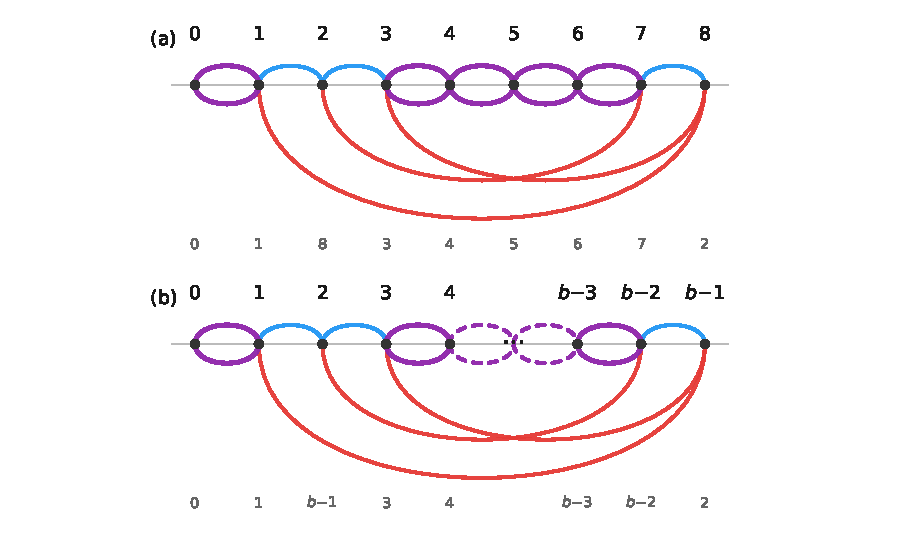
\includegraphics[width=.92\textwidth]{assets/fig_gadget_Tpb.pdf}
\caption{The odd gadget $H_{T'_b}$: (a) the instance $T'_9 = (0,1,8,3,4,5,6,7,2)$;
(b) general odd $b$, the middle of the highway elided. Conventions as in
Figure~\ref{fig:Tb}. Note the contrasts with $H_{T_b}$: vertex $0$ is a leaf (its
doubled pair $\{0,1\}$ is its only edge pair), the terminal $v_1$ sits at vertex $2$,
and the doubled run $D = \{3,\dots,b{-}2\}$ is one vertex shorter than the segment of
$H_{T_b}$ -- the relabeling that reverses the good parity from even to odd $b$.}
\label{fig:Tpb}
\end{figure}

\begin{lemma}[Highway behavior]\label{lem:oddb-segment}
Let $Q$ be a PC path in $H_{T'_b}$, $b \ge 7$ odd.
\begin{enumerate}
\item[(a)] While inside $D$, $Q$ moves monotonically in position, and $Q$ can leave
$D$ only from vertex $3$ or vertex $b-2$.
\item[(b)] Suppose $Q$ enters $D$ at one end ($3$ or $b-2$) by an edge of color $c$,
at a moment when no vertex of $D$ has yet been visited, and later leaves $D$. Then
either it leaves immediately from the entry vertex by the other external edge there,
of color $\bar c$, or it traverses all of $D$ to the far end; in the latter case its
$b - 5$ internal edges alternate colors starting with $\bar c$, and since $b$ is
\emph{odd}, $b - 5$ is \emph{even}, so the last internal edge has color $c$ and any
edge by which $Q$ then leaves $D$ has color $\bar c$.
\end{enumerate}
\end{lemma}

\begin{proof}
Identical in form to Lemma~\ref{lem:segment}, applied to $D$: (a) is immediate since a
simple path cannot reverse inside a doubled path graph and the boundary vertices of
$D$ are $3$ and $b-2$; the two external edges at each of $3$ and $b-2$ have different
colors, so an immediate exit uses the other one, of color $\bar c$. A full crossing
has $b-5$ internal edges (a path on $b-4$ vertices); the PC condition at the entry
gives the first internal edge color $\bar c$, alternation gives the last internal edge
color $c$ (as $b-5$ is even), and the PC condition at the far end forces any exit edge
to color $\bar c$.
\end{proof}

Note the parity contrast with $T_b$: the segment of Lemma~\ref{lem:segment} has $b-4$
internal edges (even iff $b$ even), while the highway here has $b-5$ (even iff $b$
odd), because the relabeling detached vertex $2$ from the doubled run. The parity that
serves even $b$ in Theorem~\ref{thm:classification} is exactly the parity that serves
odd $b$ here.

\begin{theorem}[Classification, odd gadget]\label{thm:oddb-classification}
Let $b \ge 7$ be odd. Up to reversal, the admissible visits of $H_{T'_b}$ are exactly
the following, each with the role pair shown:
\begin{center}
\begin{tabular}{clll}
\toprule
 & vertices & edges (colors) & role pair \\
\midrule
(W1) & $0$ & --- & $\{p_0, v_0\}$ \\
(W2) & $0,\ 1,\ 2$ & $\mathrm V\{0,1\},\ \mathrm P\{1,2\}$ & $\{p_0, v_1\}$ \\
(W3) & $0,\ 1,\ b-1$ & $\mathrm P\{0,1\},\ \mathrm V\{1,b{-}1\}$ & $\{v_0, p_1\}$ \\
(W4) & $2,\ 1,\ b-1$ & $\mathrm P\{1,2\},\ \mathrm V\{1,b{-}1\}$ & $\{v_1, p_1\}$ \\
(W5) & $2,\ 3,\ b-1$ & $\mathrm P\{2,3\},\ \mathrm V\{3,b{-}1\}$ & $\{v_1, p_1\}$ \\
\bottomrule
\end{tabular}
\end{center}
In particular every admissible visit has at most $3$ vertices, and $M(T'_b) = 3$,
attained by (W2)--(W5).
\end{theorem}

\begin{proof}
\emph{Each listed visit is admissible.} (W1): vertex $0$ carries $p_0$ and $v_0$ with
different port colors -- type (ii). (W2): the visit $(0,1,2)$ takes the V-copy of the
doubled pair $\{0,1\}$, then $\mathrm P\{1,2\}$; first edge
$\mathrm V \ne \pc(p_0) = \mathrm P$, last edge
$\mathrm P \ne \pc(v_1) = \mathrm V$. (W3): P-copy of $\{0,1\}$, then
$\mathrm V\{1,b-1\}$; first $\mathrm P \ne \pc(v_0)$, last
$\mathrm V \ne \pc(p_1)$. (W4): $\mathrm P\{1,2\}$ then $\mathrm V\{1,b-1\}$; first
$\mathrm P \ne \pc(v_1)$, last $\mathrm V \ne \pc(p_1)$. (W5): $\mathrm P\{2,3\}$ then
$\mathrm V\{3,b-1\}$; the same check. The role pairs are forced by the first/last edge
colors as in Theorem~\ref{thm:classification}. (Note vertex $1$ is \emph{not} a
terminal here -- it is an interior vertex of (W2)--(W4).)

\emph{No others exist.} A type-(ii) visit needs a vertex carrying two roles of
different port colors; the only vertex carrying two roles is $0 = p_0 = v_0$: (W1). A
type-(i) visit starts at a terminal vertex with a constrained first color
(Lemma~\ref{lem:reversal}(b)); the terminal vertices are $0, 2, b-1$, and the possible
(start, first color) stems are
\[
\text{(A) } (0, \mathrm V)\ [p_0], \quad
\text{(B) } (0, \mathrm P)\ [v_0], \quad
\text{(C) } (2, \mathrm P)\ [v_1], \quad
\text{(D) } (b-1, \mathrm V)\ [p_1]
\]
(vertex $2$ carries only $v_1$, which requires first color $\mathrm P$; vertex $b-1$
carries only $p_1$, requiring first color $\mathrm V$). We enumerate the PC
continuations of each stem, recording every moment the path stands at a terminal
vertex with an admissible last-edge color; since no vertex of $D$ is a terminal, a
path stranded inside $D$ ends no admissible visit.

\smallskip
\noindent\textbf{Stem (A): start $0$, first edge $\mathrm V$.} By (F0) the first edge
is the V-copy of $\{0,1\}$; at $1$, last color $\mathrm V$; no role at $1$. Continue
with a P-edge: $\{0,1\}$ is excluded ($0$ visited), so $\mathrm P\{1,2\}$; at $2$,
last color $\mathrm P$. \emph{Record:} $v_1$ at $2$ has
$\pc = \mathrm V \ne \mathrm P$: this is (W2). Continue: next $\ne \mathrm P$, so by
(F2) $\mathrm V\{2,b-2\}$, entering $D$ at $b-2$ with color $\mathrm V$, $D$
untouched. By Lemma~\ref{lem:oddb-segment}(b):
\emph{immediate exit} by $\mathrm P\{b-2,b-1\}$: at $b-1$, last color $\mathrm P$; the
only role there is $p_1$ with $\pc = \mathrm P$: not admissible. Continue: next
$\ne \mathrm P$, a V-edge at $b-1$: $\{1,b-1\}$ has $1$ visited, so
$\mathrm V\{3,b-1\}$ into $D$ at $3$; from $3$ the non-$\mathrm V$ continuations are
$\mathrm P\{2,3\}$ ($2$ visited) or the P-side of $\{3,4\}$, after which the path
ascends monotonically and strands ($b-2$ visited). \emph{Full crossing} to $3$:
arrival color $\mathrm V$, so the exit must be $\mathrm P$; the only external P-edge
at $3$ is $\{2,3\}$, with $2$ visited. Strands. \emph{Stem (A) yields exactly (W2).}

\smallskip
\noindent\textbf{Stem (B): start $0$, first edge $\mathrm P$.} By (F0) the first edge
is the P-copy of $\{0,1\}$; at $1$, last $\mathrm P$; no role. Continue with a V-edge:
$\{0,1\}$ excluded, so $\mathrm V\{1,b-1\}$; at $b-1$, last $\mathrm V$.
\emph{Record:} $p_1$ admissible: (W3). Continue: next $\ne \mathrm V$, by (F1)
$\mathrm P\{b-2,b-1\}$ into $D$ at $b-2$, color $\mathrm P$, $D$ untouched.
\emph{Immediate exit} by $\mathrm V\{2,b-2\}$: at $2$, last $\mathrm V$; role $v_1$
has $\pc = \mathrm V$: not admissible. Continue: next $\ne \mathrm V$, a P-edge
$\{1,2\}$ ($1$ visited) or $\mathrm P\{2,3\}$ into $D$ at $3$; from $3$, next
$\ne \mathrm P$ is $\mathrm V\{3,b-1\}$ ($b-1$ visited) or the V-side of $\{3,4\}$,
then monotone ascent strands ($b-2$ visited). \emph{Full crossing} to $3$: arrival
$\mathrm P$, exit must be $\mathrm V$; only $\{3,b-1\}$, with $b-1$ visited. Strands.
\emph{Stem (B) yields exactly (W3).}

\smallskip
\noindent\textbf{Stem (C): start $2$, first edge $\mathrm P$.} The P-edges at $2$ are
$\{1,2\}$ and $\{2,3\}$.
\emph{Branch $2 \to 1$:} at $1$, last $\mathrm P$; no role. Continue with a V-edge:
either $\mathrm V\{0,1\}$ -- at $0$, last $\mathrm V$; \emph{record:} $p_0$
($\pc = \mathrm P$) admissible: (W2) reversed; by (F0) the only continuation returns
to $1$, visited: dead end -- or $\mathrm V\{1,b-1\}$ -- at $b-1$, last $\mathrm V$;
\emph{record:} $p_1$ admissible: (W4). Continue: next $\ne \mathrm V$, by (F1)
$\mathrm P\{b-2,b-1\}$ into $D$ at $b-2$, color $\mathrm P$, $D$ untouched; immediate
exit by $\mathrm V\{2,b-2\}$ has $2$ visited; full crossing to $3$ arrives with
$\mathrm P$, exit must be $\mathrm V$, only $\{3,b-1\}$ with $b-1$ visited. Strands.
\emph{Branch $2 \to 3$:} enters $D$ at $3$, color $\mathrm P$, $D$ untouched.
Immediate exit by $\mathrm V\{3,b-1\}$: at $b-1$, last $\mathrm V$; \emph{record:}
$p_1$ admissible: (W5). Continue: next $\ne \mathrm V$, by (F1)
$\mathrm P\{b-2,b-1\}$ into $D$ at $b-2$ -- but $D$ is now touched (vertex $3$): the
non-$\mathrm P$ continuations at $b-2$ are $\mathrm V\{2,b-2\}$ ($2$ visited) and the
V-side of $\{b-3,b-2\}$, then monotone descent strands at $4$ ($3$ visited).
Alternatively, full crossing $3 \to b-2$ arrives with color $\mathrm P$; the exit must
be $\mathrm V$, and the only external V-edge at $b-2$ is $\{2,b-2\}$, with $2$
visited. Strands.
\emph{Stem (C) yields exactly (W2) reversed, (W4), (W5).}

\smallskip
\noindent\textbf{Stem (D): start $b-1$, first edge $\mathrm V$.} The V-edges at $b-1$
are $\{1,b-1\}$ and $\{3,b-1\}$.
\emph{Branch $b-1 \to 1$:} at $1$, last $\mathrm V$; no role. Continue with a P-edge:
either $\mathrm P\{0,1\}$ -- at $0$, last $\mathrm P$; \emph{record:} $v_0$
($\pc = \mathrm V$) admissible: (W3) reversed; the only continuation returns to $1$:
dead end -- or $\mathrm P\{1,2\}$ -- at $2$, last $\mathrm P$; \emph{record:} $v_1$
admissible: (W4) reversed. Continue: next $\ne \mathrm P$, by (F2)
$\mathrm V\{2,b-2\}$ into $D$ at $b-2$, color $\mathrm V$, $D$ untouched; immediate
exit by $\mathrm P\{b-2,b-1\}$ has $b-1$ visited; full crossing to $3$ arrives with
$\mathrm V$, exit must be $\mathrm P$, only $\{2,3\}$ with $2$ visited. Strands.
\emph{Branch $b-1 \to 3$:} enters $D$ at $3$, color $\mathrm V$, $D$ untouched.
Immediate exit by $\mathrm P\{2,3\}$: at $2$, last $\mathrm P$; \emph{record:} $v_1$
admissible: (W5) reversed. Continue: next $\ne \mathrm P$, by (F2)
$\mathrm V\{2,b-2\}$ into $D$ at $b-2$ -- $D$ touched (vertex $3$): the
non-$\mathrm V$ continuations at $b-2$ are $\mathrm P\{b-2,b-1\}$ ($b-1$ visited) and
the P-side of $\{b-3,b-2\}$, then monotone descent strands at $4$. Alternatively,
full crossing $3 \to b-2$ arrives with color $\mathrm V$; the exit must be
$\mathrm P$, only $\{b-2,b-1\}$, with $b-1$ visited. Strands.
\emph{Stem (D) yields exactly (W3) reversed, (W4) reversed, (W5) reversed.}

\smallskip
Collecting the stems: every admissible visit is one of (W1)--(W5) up to reversal, and
the maximum size is $3$.
\end{proof}

\begin{remark}[Degenerate and small cases]\label{rem:oddb-small}
For $b = 5$ the highway $D = \{3\}$ degenerates and
Lemmas~\ref{lem:oddb-inventory}--\ref{lem:oddb-segment} do not apply verbatim, but
direct enumeration confirms that the classification's \emph{shape} persists:
$T'_5 = (0,1,4,3,2)$ has admissible visits exactly $(0)$, $(0,1,2)$, $(0,1,4)$,
$(2,1,4)$, $(2,3,4)$, so $M(T'_5) = 3$. For $b = 3, 4$ no member of either gadget
family exists, and the exhaustive minima $\mu(3) = \mu(4) = 3$ are computed directly
(Appendix~\ref{sec:comp}). Note also the role pairs realized here ---
$\{p_0, v_1\}$ and $\{v_0, p_1\}$ appear, while $T_b$ forbids exactly those two ---
so the two gadget families attain the transit floor through genuinely different visit
structures.
\end{remark}

%% [E14 2026-07-28] Census appendix added (de-historicize pass): clean home for
%% the exhaustive censuses; anchors the Q1 deficient-set counts. Ledger: E14.

\section{A \texorpdfstring{$\pmin$}{rho-min} census}\label{app:census}

For $n \le 12$ the exact value of $\pmin(n)$, and the size of the \emph{deficient
set} $D(n) = \{\sigma \in S_n : \rho(\sigma) < n\}$, are known by exhaustive
enumeration (the joint $(b, \rho)$ censuses of Appendix~\ref{sec:comp}, logs
\texttt{exh7.txt}--\texttt{exh12.txt}).
%% [E22 2026-07-29] Census extended to n <= 16 from the WP-I threshold censuses
%% (research repo); |D(n)| not recorded there. Values ride P-WPI.1/.2/.4/.5.
For $13 \le n \le 16$ the value of
$\pmin(n)$ is likewise exact, by exhaustive \emph{decision censuses at a
threshold}: the search enumerates one representative per orbit of the
$\rho$-preserving symmetries of $H_\sigma$ (reversal of $\sigma$,
value-complementation, and inversion, the last of which exchanges the two
colors) and records every $\sigma$ at or below the threshold. This determines
$\pmin(n)$ and \emph{all} of its minimizers, but not the full distribution, so
$|D(n)|$ is not recorded in that range. Every minimizer found was certified by
the same independent integer-programming formulation used for
Proposition~\ref{prop:k3}; these censuses and their certificates are archived
in the research repository rather than in the ancillary artifact. For
$n \le 6$ every union is
properly-colored Hamiltonian: $D(n) = \emptyset$ and $\pmin(n) = n$, which also
follows from $f(n) = n$ for $n \le 6$ together with
Observation~\ref{obs:topcontent}.

\begin{center}
\begin{tabular}{rrrr}
\toprule
$n$ & $n!$ & $|D(n)|$ & $\pmin(n)$ \\
\midrule
$\le 6$ &  & $0$ & $n$ \\
$7$  & $5{,}040$         & $8$             & $5$ \\
$8$  & $40{,}320$        & $32$            & $6$ \\
$9$  & $362{,}880$       & $896$           & $7$ \\
$10$ & $3{,}628{,}800$   & $5{,}824$       & $8$ \\
$11$ & $39{,}916{,}800$  & $135{,}712$     & $7$ \\
$12$ & $479{,}001{,}600$ & $1{,}178{,}624$ & $8$ \\
$13$ & $6{,}227{,}020{,}800$      & --- & $9$ \\
$14$ & $87{,}178{,}291{,}200$     & --- & $10$ \\
$15$ & $1{,}307{,}674{,}368{,}000$  & --- & $9$ \\
$16$ & $20{,}922{,}789{,}888{,}000$ & --- & $10$ \\
\bottomrule
\end{tabular}
\end{center}

Two features of the table are worth recording. First, $\pmin$ is not monotone:
the values at $n = 7, 11, 15$ sit below both neighbors. Second, the deficient
sets remain a vanishing fraction of $S_n$ throughout the range where the full
distribution is known ($|D(12)|/12! \approx 0.25\%$), while their internal
structure is what the three-color census of Proposition~\ref{prop:k3} mines;
the minimizers themselves are rare (the number of $\sigma$ attaining
$\pmin(n)$ at $n = 13, 14, 15, 16$ is $290$, $2894$, $8$, $240$ respectively).
These are data, not theorems; nothing in the main text depends on this table
beyond the values $\pmin(7) = 5$ and $\pmin(8) = 6$ and the counts $|D(n)|$
quoted in Section~\ref{sec:disc}.

%% [E7 2026-07-28] The conversion lemma (old Section 3) relocated here as an
%% appendix per the E7 directive; the scrambled-ladder name (E11) and the single
%% Lovasz provenance mention live here. Ledger: E7/E8/E11.

\section{The scrambled ladder and the parameter
\texorpdfstring{$f(n)$}{f(n)}}\label{sec:conversion}

This appendix defines the graph family $G(n,\sigma)$ -- the \emph{scrambled
ladder} -- and its matching-edge parameter $f(n)$, and proves the conversion
lemma linking $f$ to $\pmin$. It is logically independent of the main text;
the growth of $f$ is posed among the open problems of Section~\ref{sec:disc}.

\begin{definition}\label{def:Gns}
For $\sigma \in S_n$, the \emph{scrambled ladder} $G(n,\sigma)$ is the graph on the
$2n$ vertices $v_0,\dots,v_{n-1}$, $u_0,\dots,u_{n-1}$, with edges:
a \emph{top path} $v_0 v_1 \cdots v_{n-1}$; a \emph{bottom path}
$u_0 u_1 \cdots u_{n-1}$; and a \emph{matching} $M = \{v_i u_{\sigma(i)} : 0\le i\le
n-1\}$. Every $v_i$ and every $u_j$ is incident to exactly one matching edge; the four
path endpoints have degree $2$ and every other vertex degree $3$. For a simple path
$\pi$ in $G(n,\sigma)$, $\mu(\pi)$ is the number of edges of $\pi$ in $M$, and
$f(n) = \min_\sigma \max_\pi \mu(\pi)$.
\end{definition}

\begin{theorem}[Conversion Lemma]\label{thm:conversion}
If $H_\sigma$ has a PC path on $k$ vertices, then $G(n,\sigma)$ has a simple path on
$2k$ vertices using exactly $k$ matching edges. Hence $\max_\pi \mu(\pi) \ge
\rho(\sigma)$ for every $\sigma$, and $f(n) \ge \pmin(n)$.
\end{theorem}

\begin{proof}
Let $w_0 w_1 \cdots w_{k-1}$ be a PC path in $H_\sigma$ with edge colors
$c_0,\dots,c_{k-2}$ alternating. Build a path $\Pi$ in $G(n,\sigma)$ on the $2k$
vertices $\{v_{w_i}\} \cup \{u_{\sigma(w_i)}\}$ as follows. If $c_0 = \mathrm P$, run
\[
  u_{\sigma(w_0)} \xrightarrow{M} v_{w_0} \xrightarrow{P} v_{w_1} \xrightarrow{M}
  u_{\sigma(w_1)} \xrightarrow{Q} u_{\sigma(w_2)} \xrightarrow{M} v_{w_2}
  \xrightarrow{P} v_{w_3} \xrightarrow{M} \cdots
\]
alternating matching edges with top/bottom path edges; if $c_0 = \mathrm V$, start
instead at $v_{w_0}$, symmetrically.

\emph{Edge validity.} A P-edge $\{w_i,w_{i+1}\}$ means $|w_i - w_{i+1}| = 1$, so
$v_{w_i} v_{w_{i+1}}$ is a top-path edge; a V-edge $\{w_i,w_{i+1}\}$ means
$|\sigma(w_i) - \sigma(w_{i+1})| = 1$, so $u_{\sigma(w_i)} u_{\sigma(w_{i+1})}$ is a
bottom-path edge. The color alternation of the PC path matches the alternation of top
versus bottom traversal in $\Pi$, so every step of $\Pi$ is a genuine edge.

\emph{Simplicity.} The top vertices $\{v_{w_i}\}$ are distinct because the $w_i$ are;
the bottom vertices $\{u_{\sigma(w_i)}\}$ are distinct because $\sigma$ is a bijection;
the two families are disjoint.

\emph{Matching count.} $\Pi$ uses one matching edge per vertex of the PC path, namely
$v_{w_i} u_{\sigma(w_i)}$ for $0\le i<k$: a total of $k$.

Taking $\pi=\Pi$ gives $\max_\pi\mu(\pi)\ge\rho(\sigma)$ for each $\sigma$; the
minimum over $\sigma$ gives $f(n)\ge\pmin(n)$.
\end{proof}

The conversion is one-directional: a path in $G(n,\sigma)$ that uses two consecutive
edges of the same path (top or bottom) has no PC-path preimage, so the inequality
$f(n)\ge\pmin(n)$ cannot be reversed. This is the precise sense in which the negative
result for $\pmin$ (Theorem~\ref{thm:main-intro}) does not transfer to $f$.

What is known about $f$ beyond the conversion inequality is quickly stated.
The strongest lower bound we are aware of is $f(n) \ge 0.1\, n^{4/5}$, which is
Lemma~8 of \cite{NSTW25} (there stated for an arbitrary matching between two
vertex-disjoint paths; suppressing unmatched vertices makes the two
formulations equivalent), resting on the circumference theorem of \cite{LYZ18};
Observation~\ref{obs:topcontent} gives $f(n) \le n - 1$ for $n \ge 7$, and the
first exact values appear in Section~\ref{sec:disc}. Historically, this
construction is how the problem of this paper arose: it relates to the
Hamiltonicity question of Lov\'asz \cite{Lov70} for vertex-transitive graphs
through Lemma~8 of \cite{NSTW25}; although that route is now closed --
sublinear-expander methods reach the same $n^{2/3-o(1)}$ target without the
matching structure \cite{BCPS26} -- it was the initial motivation for our
reduction into the study of $\pmin(n)$.

\section{Computational verification}\label{sec:comp}

The asymptotic theorems and their constants are proved without computation; the
computer-assisted claims are the small-size base cases $b \in \{4,5\}$ of
Proposition~\ref{prop:floor-upper}, the spectrum data of Remark~\ref{rem:spectrum},
the $\pmin$ census of Appendix~\ref{app:census}, and the $k$-color and
matching-content values of Section~\ref{sec:disc}. This section specifies the
computations that independently verify the constructions and supply the exact
small-case values, and records the empirical sharpness of the families.
\textbf{All code, command lines, and output logs are provided as ancillary files with
this submission} (directory \texttt{code/} in the repository; \texttt{code/README.md}
maps each claim
below to a script and a log, and \texttt{code/MANIFEST.sha256} lists SHA-256 checksums).

\paragraph{Algorithm.} The basic object is an exact longest-PC-path search. Its state
space is the set of triples (\emph{visited set}, \emph{current vertex}, \emph{last edge
color}); the initial states are all $(\{x, w\}, w, c)$ over edges $\{x, w\}$ of color
$c$; a transition extends a state by an unvisited neighbor along an edge of the other
color. The legal future extensions of a partial PC path depend only on its state, so
distinct PC paths reaching the same state may be identified without loss; $\rho(\sigma)$
is then the maximum cardinality of the visited set over all \emph{reachable} states,
computed by an exhaustive search that visits every reachable state once (a memo set of
states; no pruning). The method is exact by construction; its cost is the number of
reachable states. That number is exponential in general -- on unstructured instances we
used the method only for $n \le 19$ -- but is small on the structured families here,
because the gadget admits relatively few reachable states: for $\sigma_{a,b}$ we measure
$57{,}066$
reachable states at $n = 80$, $5{,}012{,}186$ at $n = 600$, and $7{,}273{,}586$ at
$n = 720$ (the logs report the count for every table row). The constrained variants
computing $M(\pi)$ (fixed start/end terminals and first/last colors) are the same search
with the initial and accepting states restricted.

\paragraph{Implementations.} Three independent implementations were used: a plain
recursive enumerator and a memoized iterative one (both Python, in the artifact), which
agree on $300$ random permutations of sizes $4$--$8$; and an independently written C++
solver (also in the artifact), which agrees with the
Python solvers on every instance checked by both, including exact values of
$\rho(\sigma_{a,b})$ at $(a,b) \in \{(6,8), (5,10), (4,12)\}$. In addition, the
artifact contains a
\emph{minimal independent verifier} (\texttt{verify\_M.py}, about $100$ lines, written
directly from Definition~\ref{def:M} with no shared code), which re-derives $M(T_b)$ and
the complete list of admissible visits by brute force for $b \le 14$.

\paragraph{Verified statements.} Each item states the claim, its range, and its log.
\begin{enumerate}
\item \textbf{Census anchors} (\texttt{search\_small.log}): $\pmin(7) = 5$ and
$\pmin(8) = 6$ by full enumeration of $S_7, S_8$ with the Python solvers,
independently of the C++ censuses of item~4; see Appendix~\ref{app:census}.
%% [E25 cut 2026-07-30] Item "Classification" (verify_M checks of thm:classification
%% + odd-b values) removed: reassurance of a fully proved theorem; the intro's
%% F1 clause went with it. verify_M.py itself stays (Implementations paragraph).
%% [E25 cut 2026-07-30] Item "The family at scale" (M(T_b)=3 to b=100) removed:
%% pure reassurance of thm:classification, which proves it for all even b.
\item \textbf{Optimality of the gadget at small sizes} (\texttt{search\_small.log}):
full enumeration of $S_b$ for $4 \le b \le 9$ gives $\min_{\pi \in S_b} M(\pi) = 3$ in
every case; no gadget of size $\le 9$ beats transit number $3$.
%% [E25 cut 2026-07-30] Item "Explicit lower-bound path" removed: reassurance of the
%% fully proved prop:lower (twin of the E20-F2 in-proof sentence cut).
\item \textbf{Exact values} (\texttt{endtoend.log}, \texttt{bigtable.log}): for
$\sigma_{a,b}$:

\begin{center}
\begin{tabular}{rrrrrrr}
\toprule
$a$ & $b$ & $n$ & $\rho$ (exact) & $2a{+}2b{-}4$ & $4a{+}2b$ & $\rho/n$ \\
\midrule
10 & 8  & 80  & 32 & 32 & 56  & 0.400 \\
12 & 8  & 96  & 36 & 36 & 64  & 0.375 \\
12 & 12 & 144 & 44 & 44 & 72  & 0.306 \\
16 & 12 & 192 & 52 & 52 & 88  & 0.271 \\
20 & 12 & 240 & 60 & 60 & 104 & 0.250 \\
16 & 16 & 256 & 60 & 60 & 96  & 0.234 \\
24 & 16 & 384 & 76 & 76 & 128 & 0.198 \\
20 & 20 & 400 & 76 & 76 & 120 & 0.190 \\
30 & 16 & 480 & 88 & 88 & 152 & 0.183 \\
24 & 20 & 480 & 84 & 84 & 136 & 0.175 \\
30 & 20 & 600 & 96 & 96 & 160 & 0.160 \\
36 & 20 & 720 & 108 & 108 & 184 & 0.150 \\
\bottomrule
\end{tabular}
\end{center}

Every exact value equals $2a + 2b - 4$ and sits inside the proven window
$[2a{+}2b{-}7,\ 4a{+}2b]$ of \eqref{eq:twosided}; the two rows at $n = 480$ (differing
in $\rho$) illustrate that $\rho(\sigma_{a,b})$ tracks $a$ and $b$ separately, not just
their product.
\item \textbf{Exhaustive small-$n$ statistics} (\texttt{logs/exh7.txt}--%
\texttt{exh12.txt}, C++ solver): the joint distribution of $(b(\sigma), \rho(\sigma))$
over all of $S_n$ for $7 \le n \le 12$, the source of the $\pmin$ census of
Appendix~\ref{app:census} and of the deficient-set counts $|D(n)|$ quoted in
Section~\ref{sec:disc}; at $n = 12$ this enumerates all $479{,}001{,}600$
permutations.
%% [E25 cut 2026-07-30] Item "Landscape" (probe.py, exploratory) removed: orphan --
%% no claim in the paper cited it; process narrative.
%% [E25 cut 2026-07-30] Item "The transit-floor construction" (verify_floor) removed:
%% reassurance of the fully proved thm:floor-lower; the rem:floor-consequences
%% validation sentence (E20-F3) went with it.
\item \textbf{The odd gadget and the spectrum} (\texttt{verify\_oddb.log},
\texttt{verify\_spectrum.log}): the inventory, highway and crossing claims of
Appendix~\ref{app:oddb} confirmed uniformly for odd $b \in \{7, 9, \dots, 21\}$, and
$M(T'_b) = 3$ there and at the degenerate $b = 5$; as positive control the same
checker reproduces $M(T_b) = 3$ (even $b$) and $M(T_b) = b$ (odd $b$) for the
even-gadget family. Separately, exhaustive computation of $M(\pi)$ for every
$\pi \in S_b$, $2 \le b \le 8$, yields $\mu(2) = 2$, $\mu(b) = 3$ for $3 \le b \le 8$,
and the attained spectra of Remark~\ref{rem:spectrum}
(\texttt{verify\_spectrum.log}).
\end{enumerate}

Every item is exhaustive or certified within its stated range and reproducible by
running the listed scripts.

The $k$-color and matching-content computations behind
Proposition~\ref{prop:k3}, Observation~\ref{obs:topcontent}, and the exact
$f(n)$ values are likewise included in the ancillary artifact: a three-color
extension of the search engine with the deficient-set/coset-triangle reduction
(\texttt{k3.cpp}) and an independent integer-programming certification of all
twelve witnesses (\texttt{cpsat\_rho3.py}); an exact bitmask dynamic program
for $\max_\pi \mu(\pi)$ over $G(n,\sigma)$ (\texttt{fmu.cpp}; validated
against a direct search on all of $S_n$ for $n \le 7$, and against the
conversion inequality $\max_\pi \mu \ge \rho$ pointwise on every permutation
processed); an integer-programming formulation for $\max_\pi \mu$ used for
the structured instances (\texttt{fmu\_cpsat.py}, optimality certified in all
reported cases).

\section*{Acknowledgments}

This paper merges and supersedes the author's two earlier notes on this problem,
and extends them with the transit-floor theorem (Section~\ref{sec:floor}) and the
open-problems data of Section~\ref{sec:disc}, obtained in a follow-up research
campaign. The proofs and computations were
AI-assisted by Claude, under the Periapsis research structure.
%% [E20 2026-07-29] "checkable without trusting either the author or the
%% assistant" stance removed (not appropriate for publication); the factual
%% checkability list below is kept.
The central case analyses are classifications
(Theorems~\ref{thm:classification} and~\ref{thm:oddb-classification}) and elementary
matching arguments (Theorem~\ref{thm:floor-lower}) whose every step is locally
verifiable; every computational claim is reproducible from the ancillary artifact,
which includes independent verifiers written directly from the definitions.
%% [E24 cut 2026-07-30] "second proof in Appendix A" clause removed with app:trap.
%% [E20 2026-07-29] "unrefereed preprint" sentence cut (same stance-genre as the
%% removed trust wording; false upon acceptance).

%% [E20 2026-07-29] References reordered by approximate relevance: the
%% alternating-path literature (the paper's field) first; the f(n)/provenance
%% cluster (appendix-only) after; Lovasz last.
\begin{thebibliography}{9}

\bibitem{BJG97}
J.~Bang-Jensen and G.~Gutin,
\emph{Alternating cycles and paths in edge-coloured multigraphs: a survey},
Discrete Math.\ \textbf{165--166} (1997), 39--60.

\bibitem{GK09}
G.~Gutin and E.~J.~Kim,
\emph{Properly coloured cycles and paths: results and open problems},
in: Graph Theory, Computational Intelligence and Thought,
Lecture Notes in Comput.\ Sci.\ 5420, Springer, 2009, 200--208.

\bibitem{ABMMM10}
A.~Abouelaoualim, V.~Borozan, Y.~Manoussakis, C.~Martinhon, and R.~Muthu,
\emph{Properly colored paths in edge-colored graphs},
Discrete Math.\ \textbf{310} (2010), 1610--1620.

\bibitem{NSTW25}
S.~Norin, R.~Steiner, S.~Thomass\'e, and P.~Wollan,
\emph{Small hitting sets for longest paths and cycles},
arXiv:2505.08634, 2025.

\bibitem{LYZ18}
Q.~Liu, X.~Yu, and Z.~Zhang,
\emph{Circumference of 3-connected cubic graphs},
J.~Combin.\ Theory Ser.~B \textbf{128} (2018), 134--159.

\bibitem{BCPS26}
M.~Buci\'c, M.~Christoph, A.~Pokrovskiy, and R.~Steiner,
\emph{Towards the Lov\'asz conjecture via sublinear expanders},
arXiv:2606.09742, 2026.

\bibitem{Lov70}
L.~Lov\'asz,
Problem 11, in:
\emph{Combinatorial Structures and their Applications}
(Proc.\ Calgary Internat.\ Conf., 1969),
Gordon and Breach, New York, 1970, p.~497.

\end{thebibliography}

\end{document}
